\chapter{Error propagation in depletion calculations}
In the \gls{MC} depletion analyses, the uncertainties on predicted isotopic 
composition are caused by two primary factors: stochastic uncertainty in 
the computed flux and uncertainty in the nuclear data (cross sections, fission 
yields, decay constants). In \gls{MC} reactor physics software, the stochastic 
uncertainty of single burnup step is superposed with errors, propagated 
throughout calculation from previous steps. Over time, these errors 
accumulate, and cumulative error in the predicted number density might be 
significant for the lifetime-long fuel depletion calculations.

Takeda \emph{et al.} first proposed a method to evaluate uncertainty of the 
number density in the \gls{MC} simulations applying the sensitivities of the 
burnup matrix to cross sections and number densities. Takeda and colleagues 
propagated covariances of the cross sections and obtained the number 
density uncertainty due to the cross section error of about 4\% for major 
heavy isotopes ($^{235}$U, $^{239}$Pu, $^{241}$Pu) after 400-day 
\gls{MC} burnup calculation for homogeneous model of fast reactor. Notably, 
the number density uncertainty due to the stochastic error in MCNP was 
much lower: about 0.03\% for $^{241}$Pu, 0.02\% for $^{235}$U, and $<0.004$\% 
for $^{238}$U. The Takeda model showed that statistical error contribution to 
the total error in number densities of major heavy isotopes and \glspl{FP} is 
less than 1\% \cite{takeda_estimation_1999}. Finally, substantial neutron 
population ($N$) increase can theoretically reduce the stochastic error to 
zero but it is enormously expensive due to slow convergence ($O(\sqrt{N})$) of 
Monte Carlo method.

Garcia-Herranz \emph{et al.} used MCNP and in-house code ACAB to analyze the 
uncertainties on the nuclide inventory based on random samplinq technique for 
single, spherical fuel element (``pebble") contained coated PuO$_2$ fuel 
particle. The random sampling or ``brute force" method is the multi-step 
scheme of stochastic neutronics and depletion calculation could be considered 
as a single process with (nuclear data) and output (final number densities). 
Authors performed a simultaneous random sampling of all the cross 
sections\footnote{Authors assumed that the influence of uncertainties in decay 
constants, fission yields and other input parameters are negligible.} 1000 
times and obtained the distributions of the isotopic inventory. Relative error 
of the final number density for 1200-day fuel cycle (800 MWg/kgHM burnup) due 
to cross section uncertainties was reported in range from 7\% (for $^{244}$Pu) 
to 46\% (for $^{242}$Pu) and found to be independent of neutron history size. 
In contrast, similar characteristic but only due to stochastic error for 
reasonably large neutron history was less than 0.15\% 
\cite{garcia-herranz_propagation_2008}. Thus, random sampling Monte Carlo 
results by Garcia-Herranz \emph{et al.} agreed with Takeda statement that 
nuclear data is the major source of uncertainty; stochastic error contribution 
to the total nuclear density error is negligibly small ($<1$\%) and might be 
reduced to almost further by substantially increasing neutron histories.

In similar vein, Radaideh \emph{et al.} used SCALE 6.2 
\cite{rearden_scale_2018} to quantify the uncertainty in nuclide concentration 
in \gls{BWR} 10$\times$10 assembly due to uncertainties in neutron cross 
sections, fission yield, and decay data \cite{radaideh_uncertainty_2018}. The 
Radaideh model used 56-group covariance library in deterministic code TRITON 
(2D) depletion calculations and, hence, introduced no stochastic error in the 
flux calculations. That work used 500 random samples in 1174-day TRITON 
depletion calculation and reported number density uncertainty between 0.14\% 
for $^{238}$U and 6.56\% for $^{238}$Pu \cite{radaideh_novel_2019-1}. This 
approach
benefits from Sampler module available in the SCALE package and 
can be used by SCALE users across the world.

All listed research efforts studied simplified, pin-cell or single-assembly 
models of conventional \gls{LWR} and considered nuclear data uncertainty for 
following elements: hydrogen, oxygen, zirconium, uranium, and plutonium. The 
nuclear data for these elements have relatively low uncertainty because it was 
measured many times for myriad weapon and non-weapon applications. However, 
the \gls{TAP} \gls{MSR} and many other designs rely on other elements such as 
lithium and fluorine which have relatively high cross section covariances. 
Effect of $^6$Li, $^7$Li, and $^{19}$F nuclear data uncertainty on final 
isotopic composition uncertainty was never studied before. This chapter seeks 
to estimate the uncertainties on predicted isotopic composition for the 
\gls{TAP} \gls{MSR} during lifetime-long depletion simulations.

In this chapter, the uncertainty in the fuel salt composition will be 
investigated for two different sources of uncertainty separately. The 
uncertainty in the nuclides inventory due to the transport problem statistical 
error is evaluated using random sampling technique using Serpent Monte Carlo 
code. By changing the code's initial random number seed, the data produce by 
1000 runs is used to investigate statistical error in multiplication factor 
($k_{eff}$) and number density of major isotopes. The uncertainty in depleted 
fuel salt composition due to nuclear data uncertainties - a major part of 
nuclear density uncertainty - is determined using SCALE/Sampler sequence in 
conjunction with TRITON (2D, deterministic code). Uncertainties in nuclear
data (e.g., neutron cross sections, fission yields, decay constants) are 
propagated into the response of
interest (fuel salt isotopic composition) by 
generating a large number of samples with perturbed nuclear data. The two 
approaches are demonstrated
using the \gls{TAP} reactor model.



\section{Stochastic uncertainty in depleted fuel composition}

\begin{figure}[hbp!] % replace 't' with 'b' to 
	\centering
	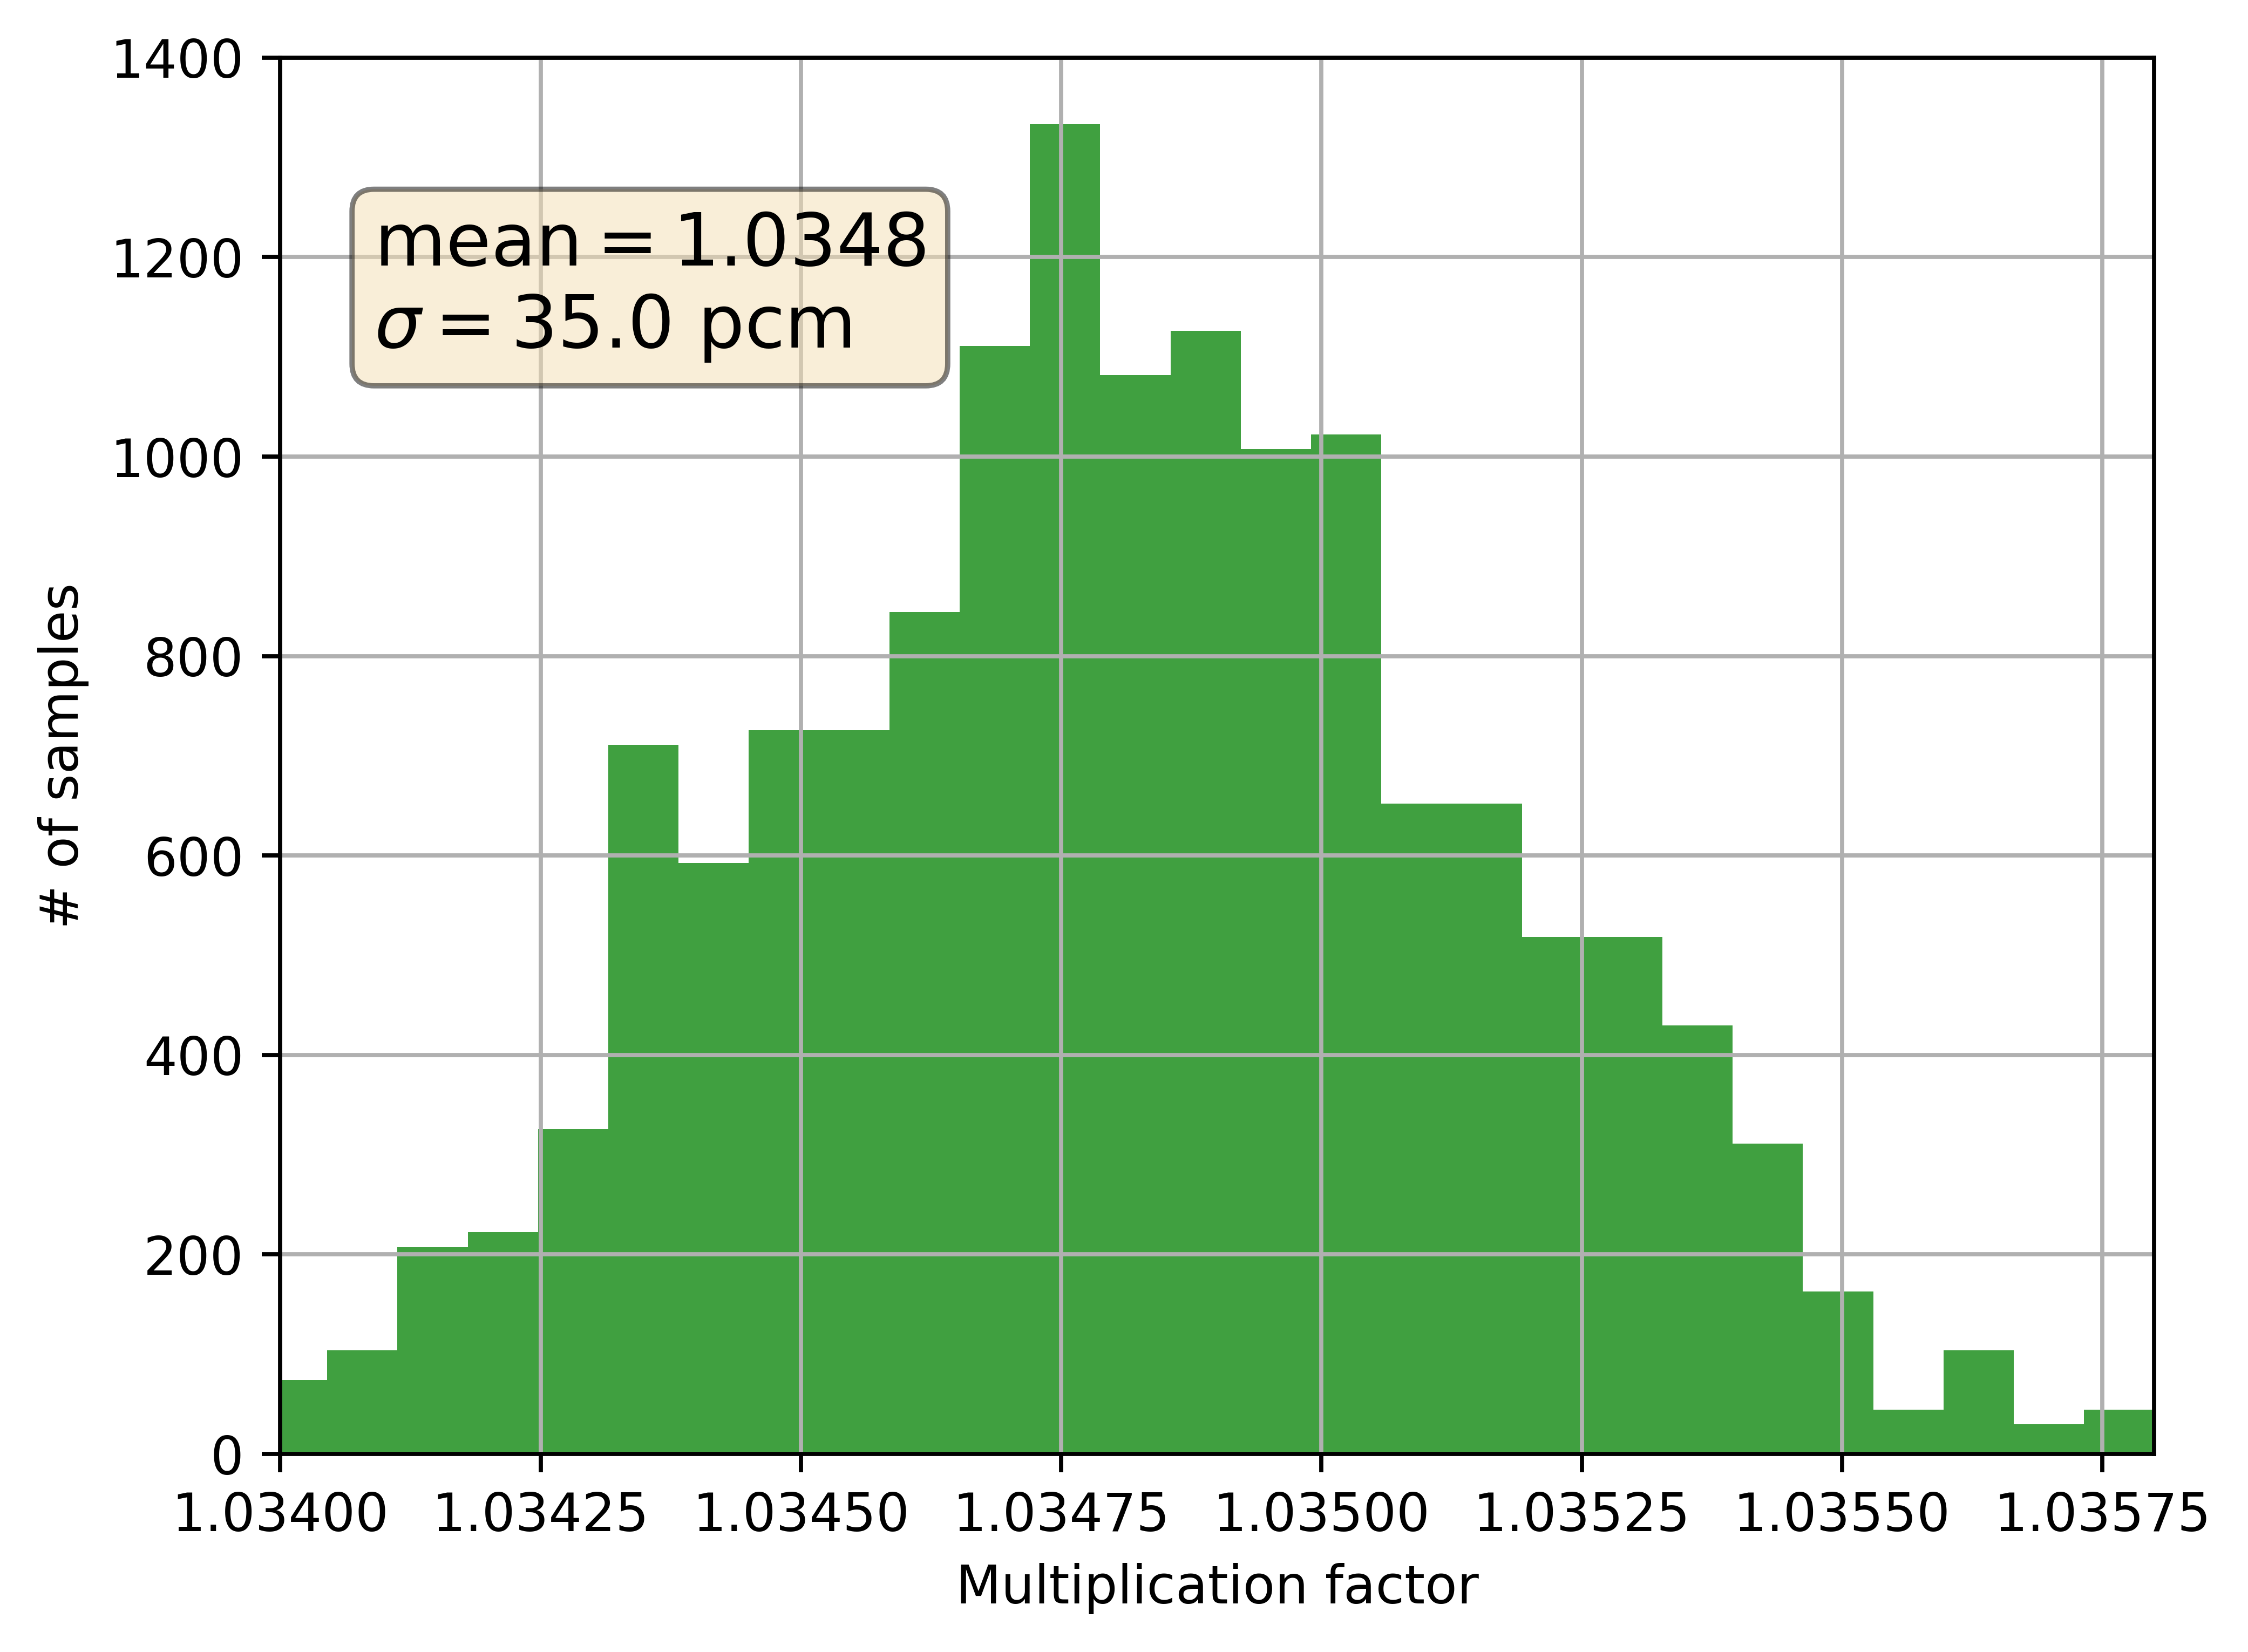
\includegraphics[width=0.8\textwidth]{uq/endf_serpent_keff_boc_for_tap.png}
	\caption{Caption here.}
	\label{fig:11}
\end{figure}
\begin{figure}[hbp!] % replace 't' with 'b' to 
	\centering
	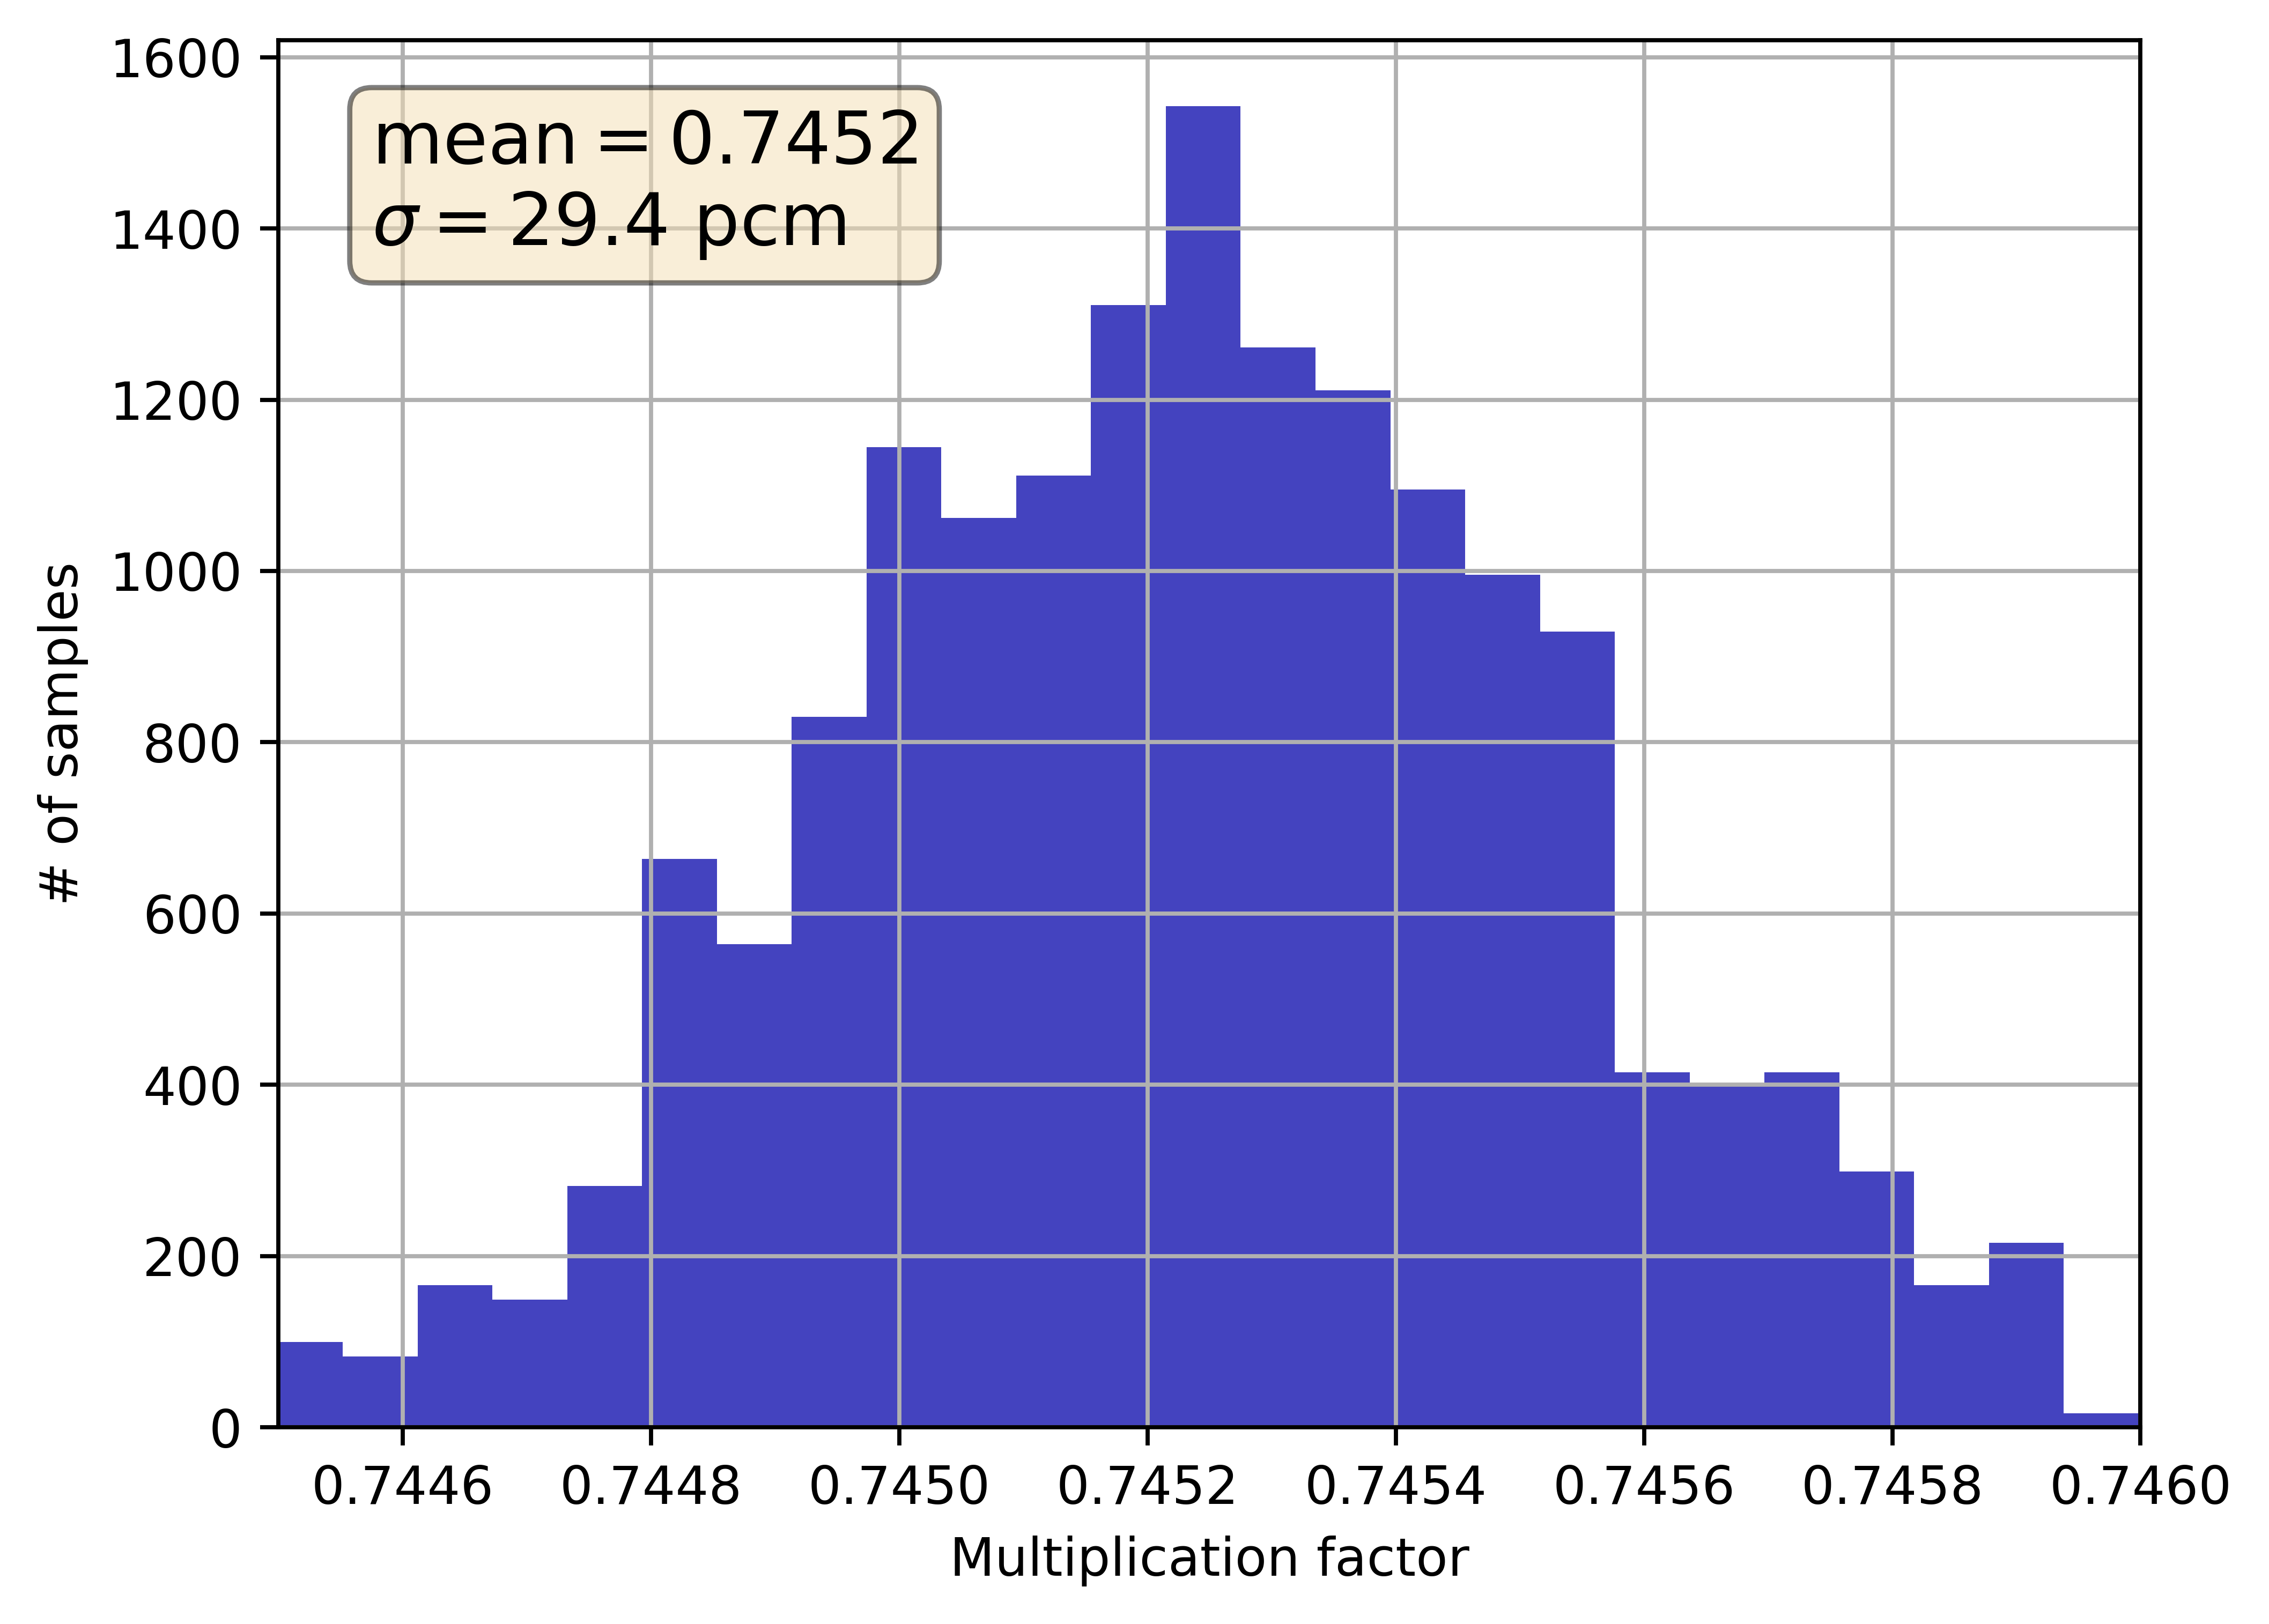
\includegraphics[width=0.8\textwidth]{uq/endf_serpent_keff_eoc_for_tap.png}
	\caption{Caption here.}
	\label{fig:22}
\end{figure}
\begin{figure}[hbp!] % replace 't' with 'b' to 
	\centering
	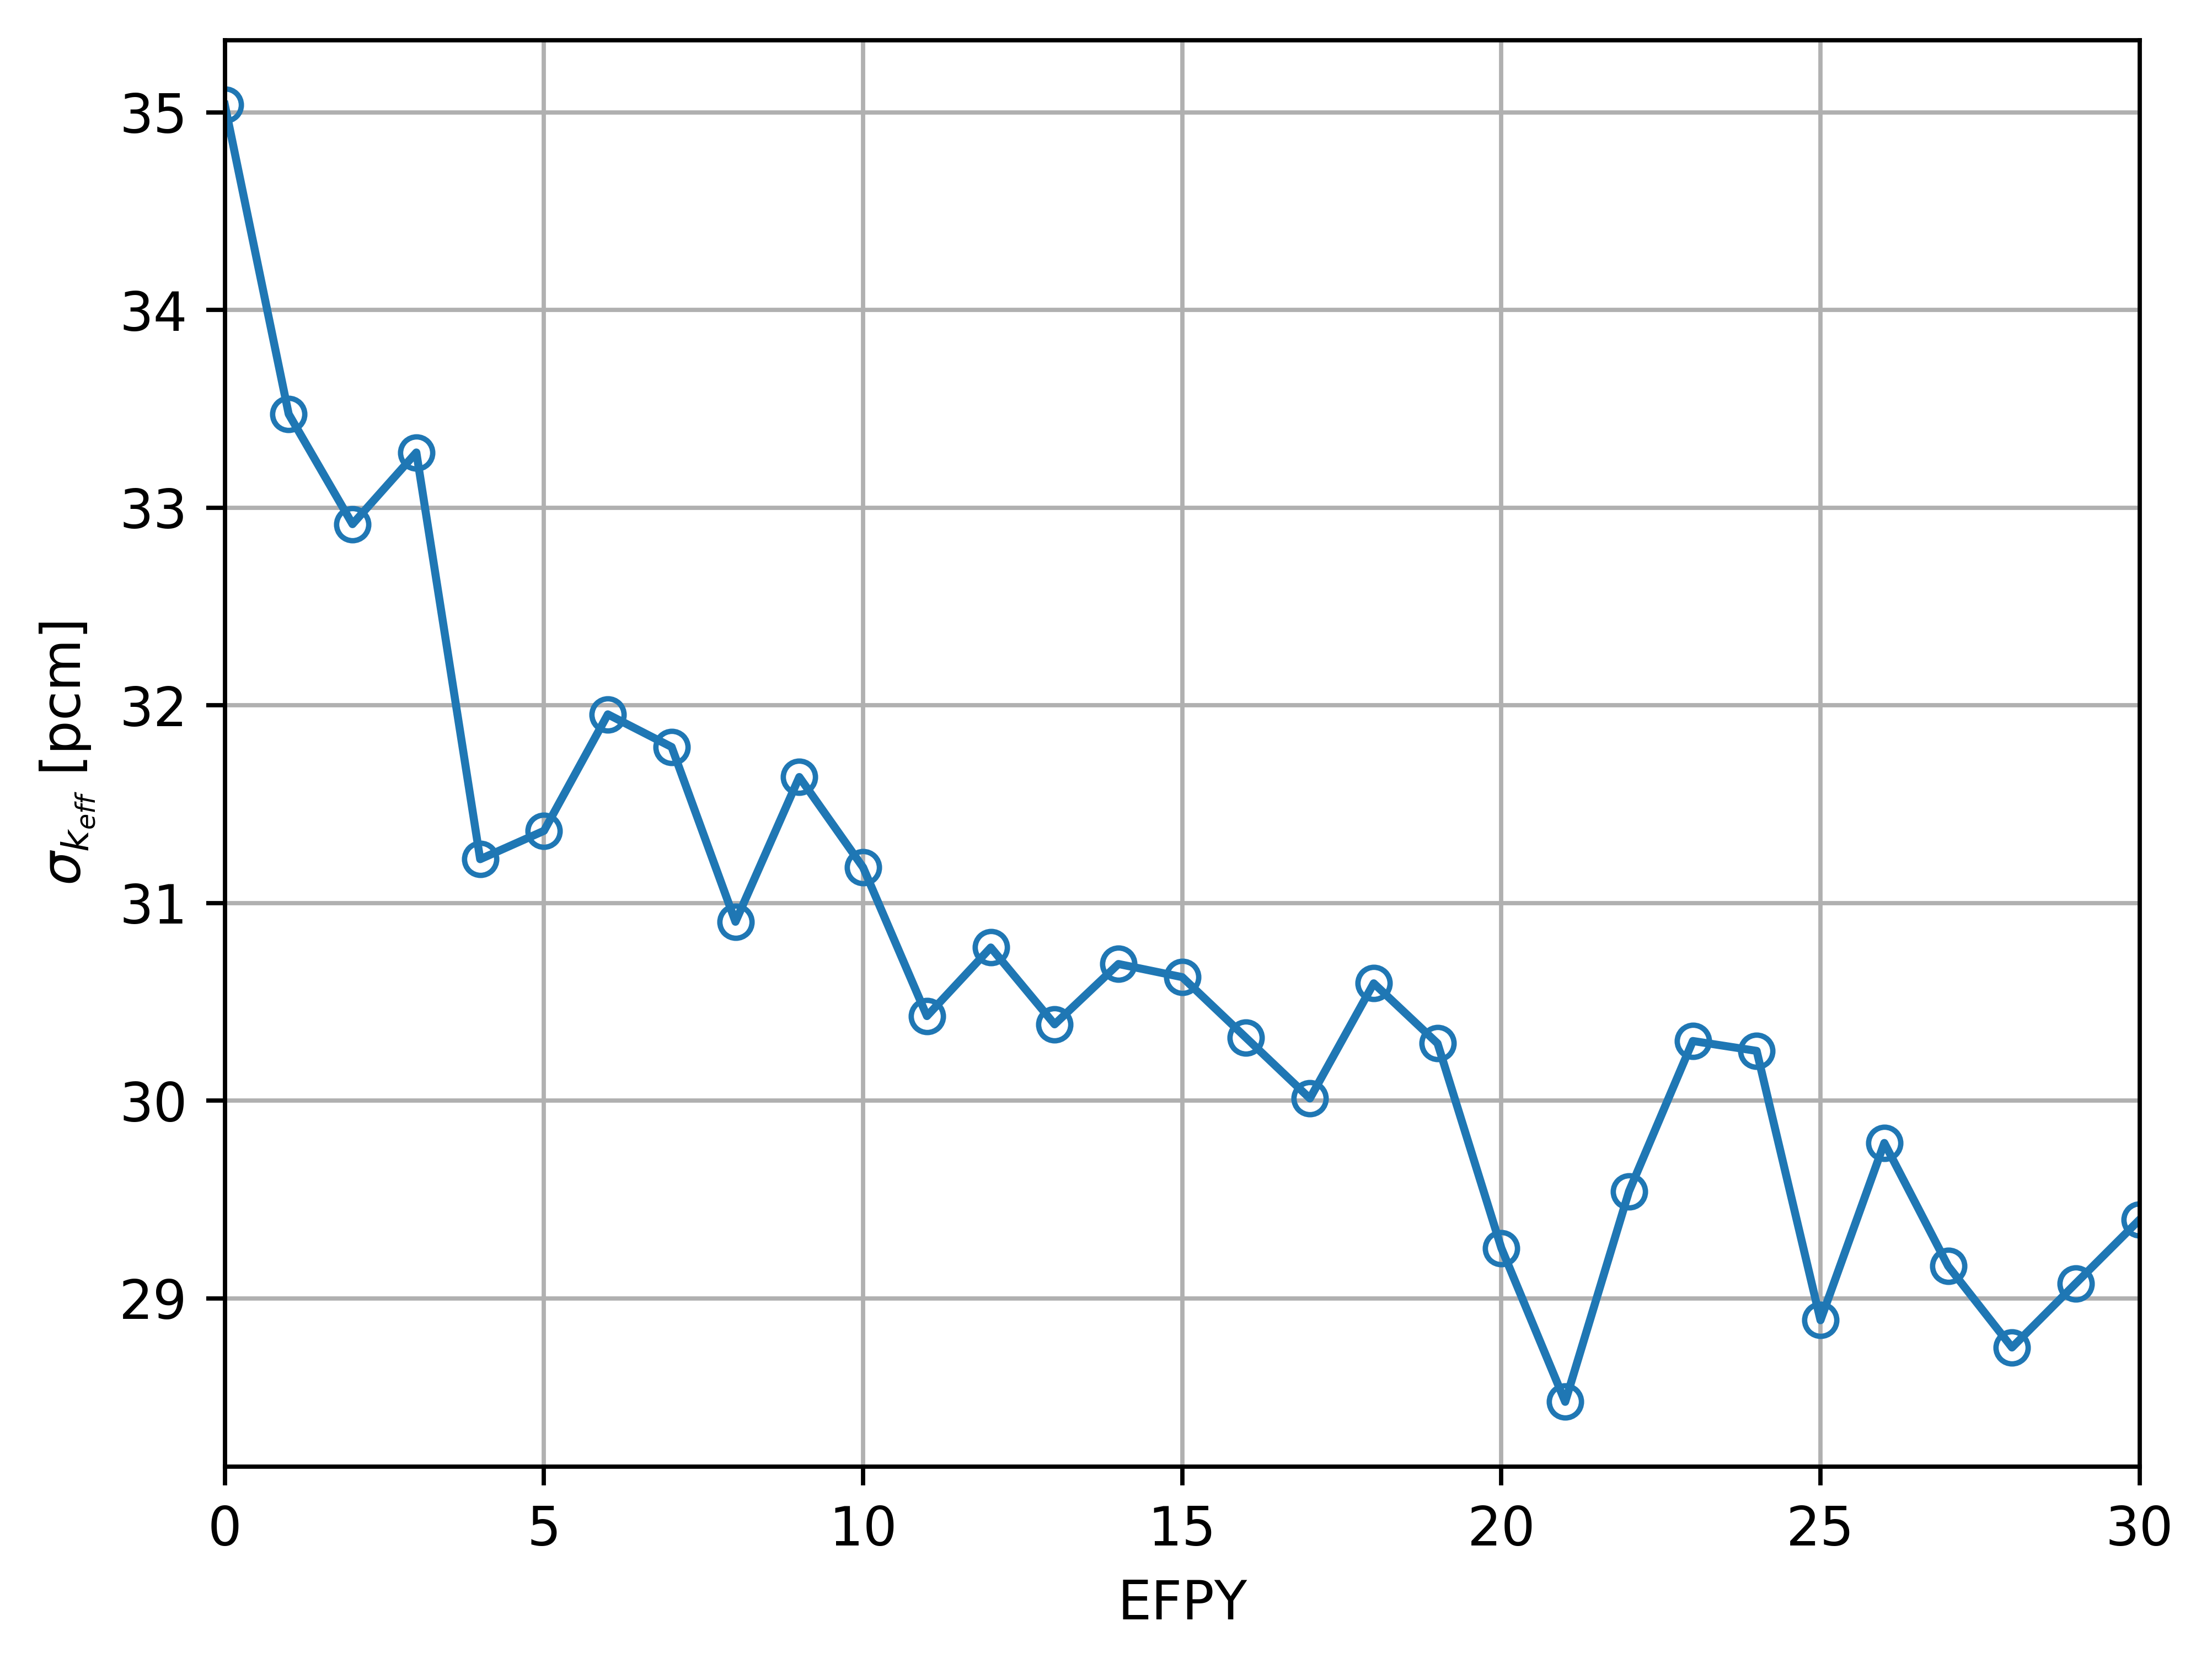
\includegraphics[width=0.8\textwidth]{uq/endf_serpent_keff_dynamics_for_tap.png}
	\caption{Caption here.}
	\label{fig:33}
\end{figure}
\begin{figure}[hbp!] % replace 't' with 'b' to 
	\centering
	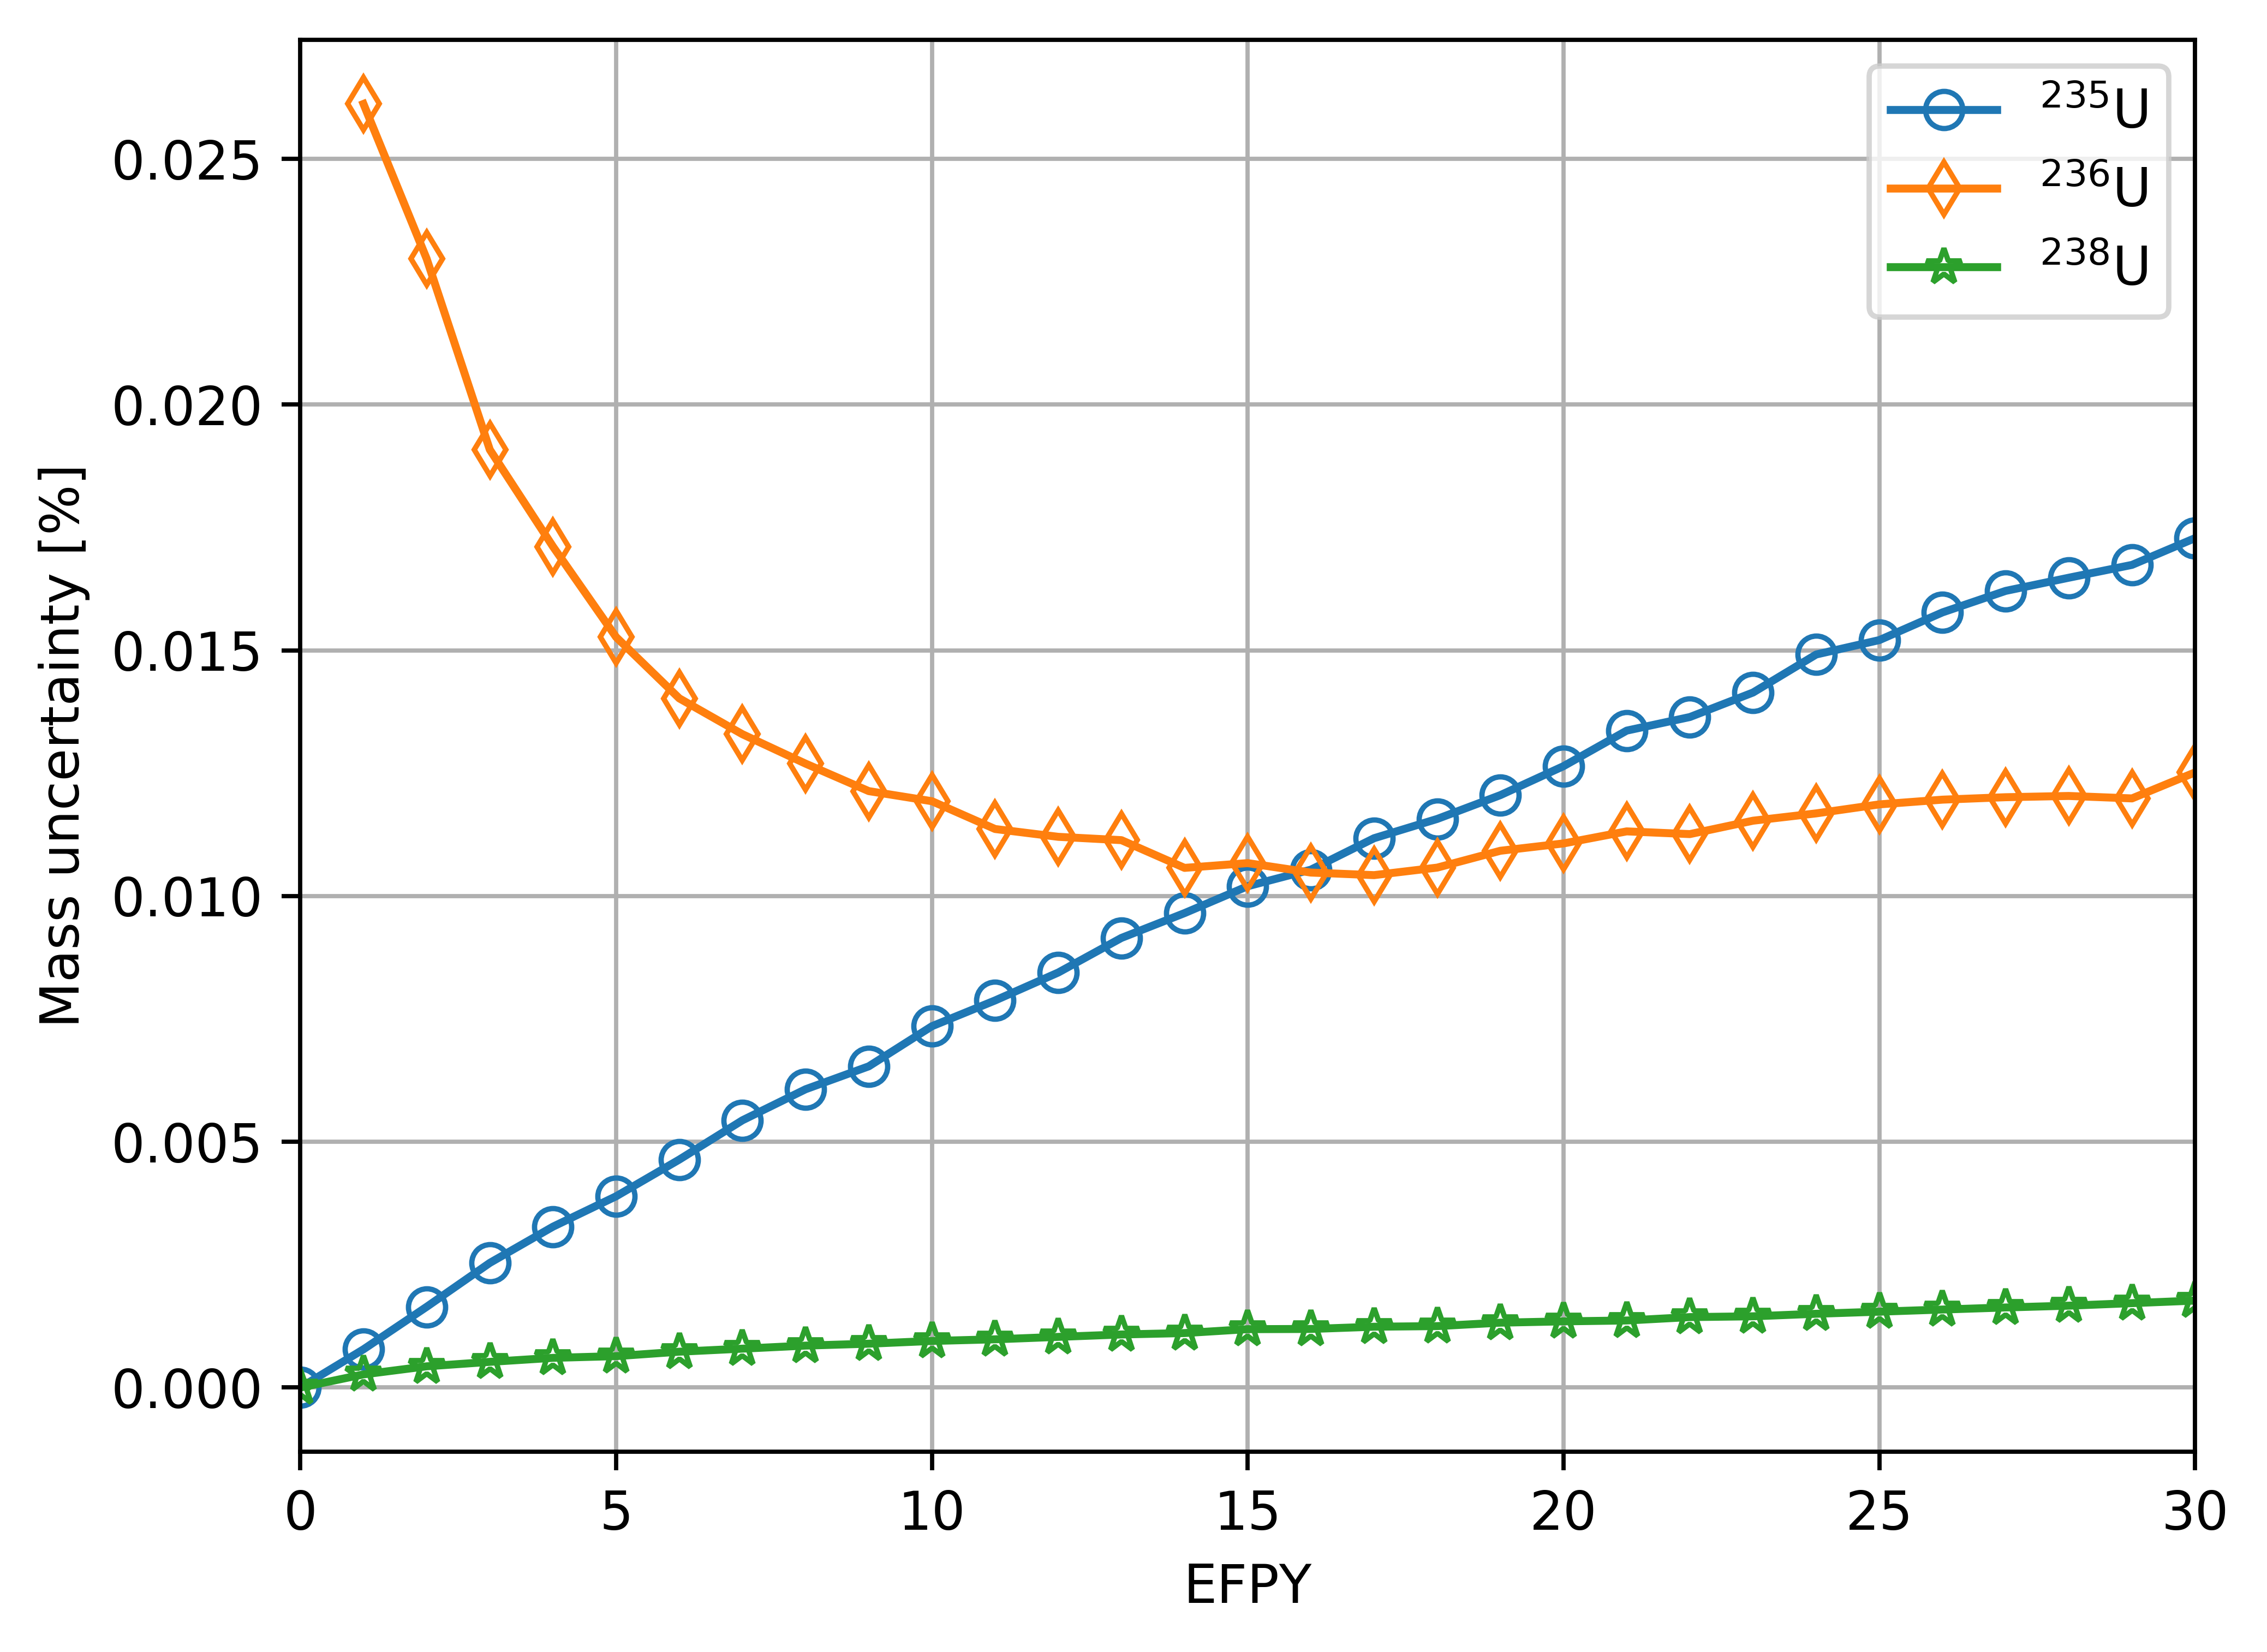
\includegraphics[width=0.8\textwidth]{uq/serpent_mass_std_u.png}
	\caption{Caption here.}
	\label{fig:44}
\end{figure}
\begin{figure}[hbp!] % replace 't' with 'b' to 
	\centering
	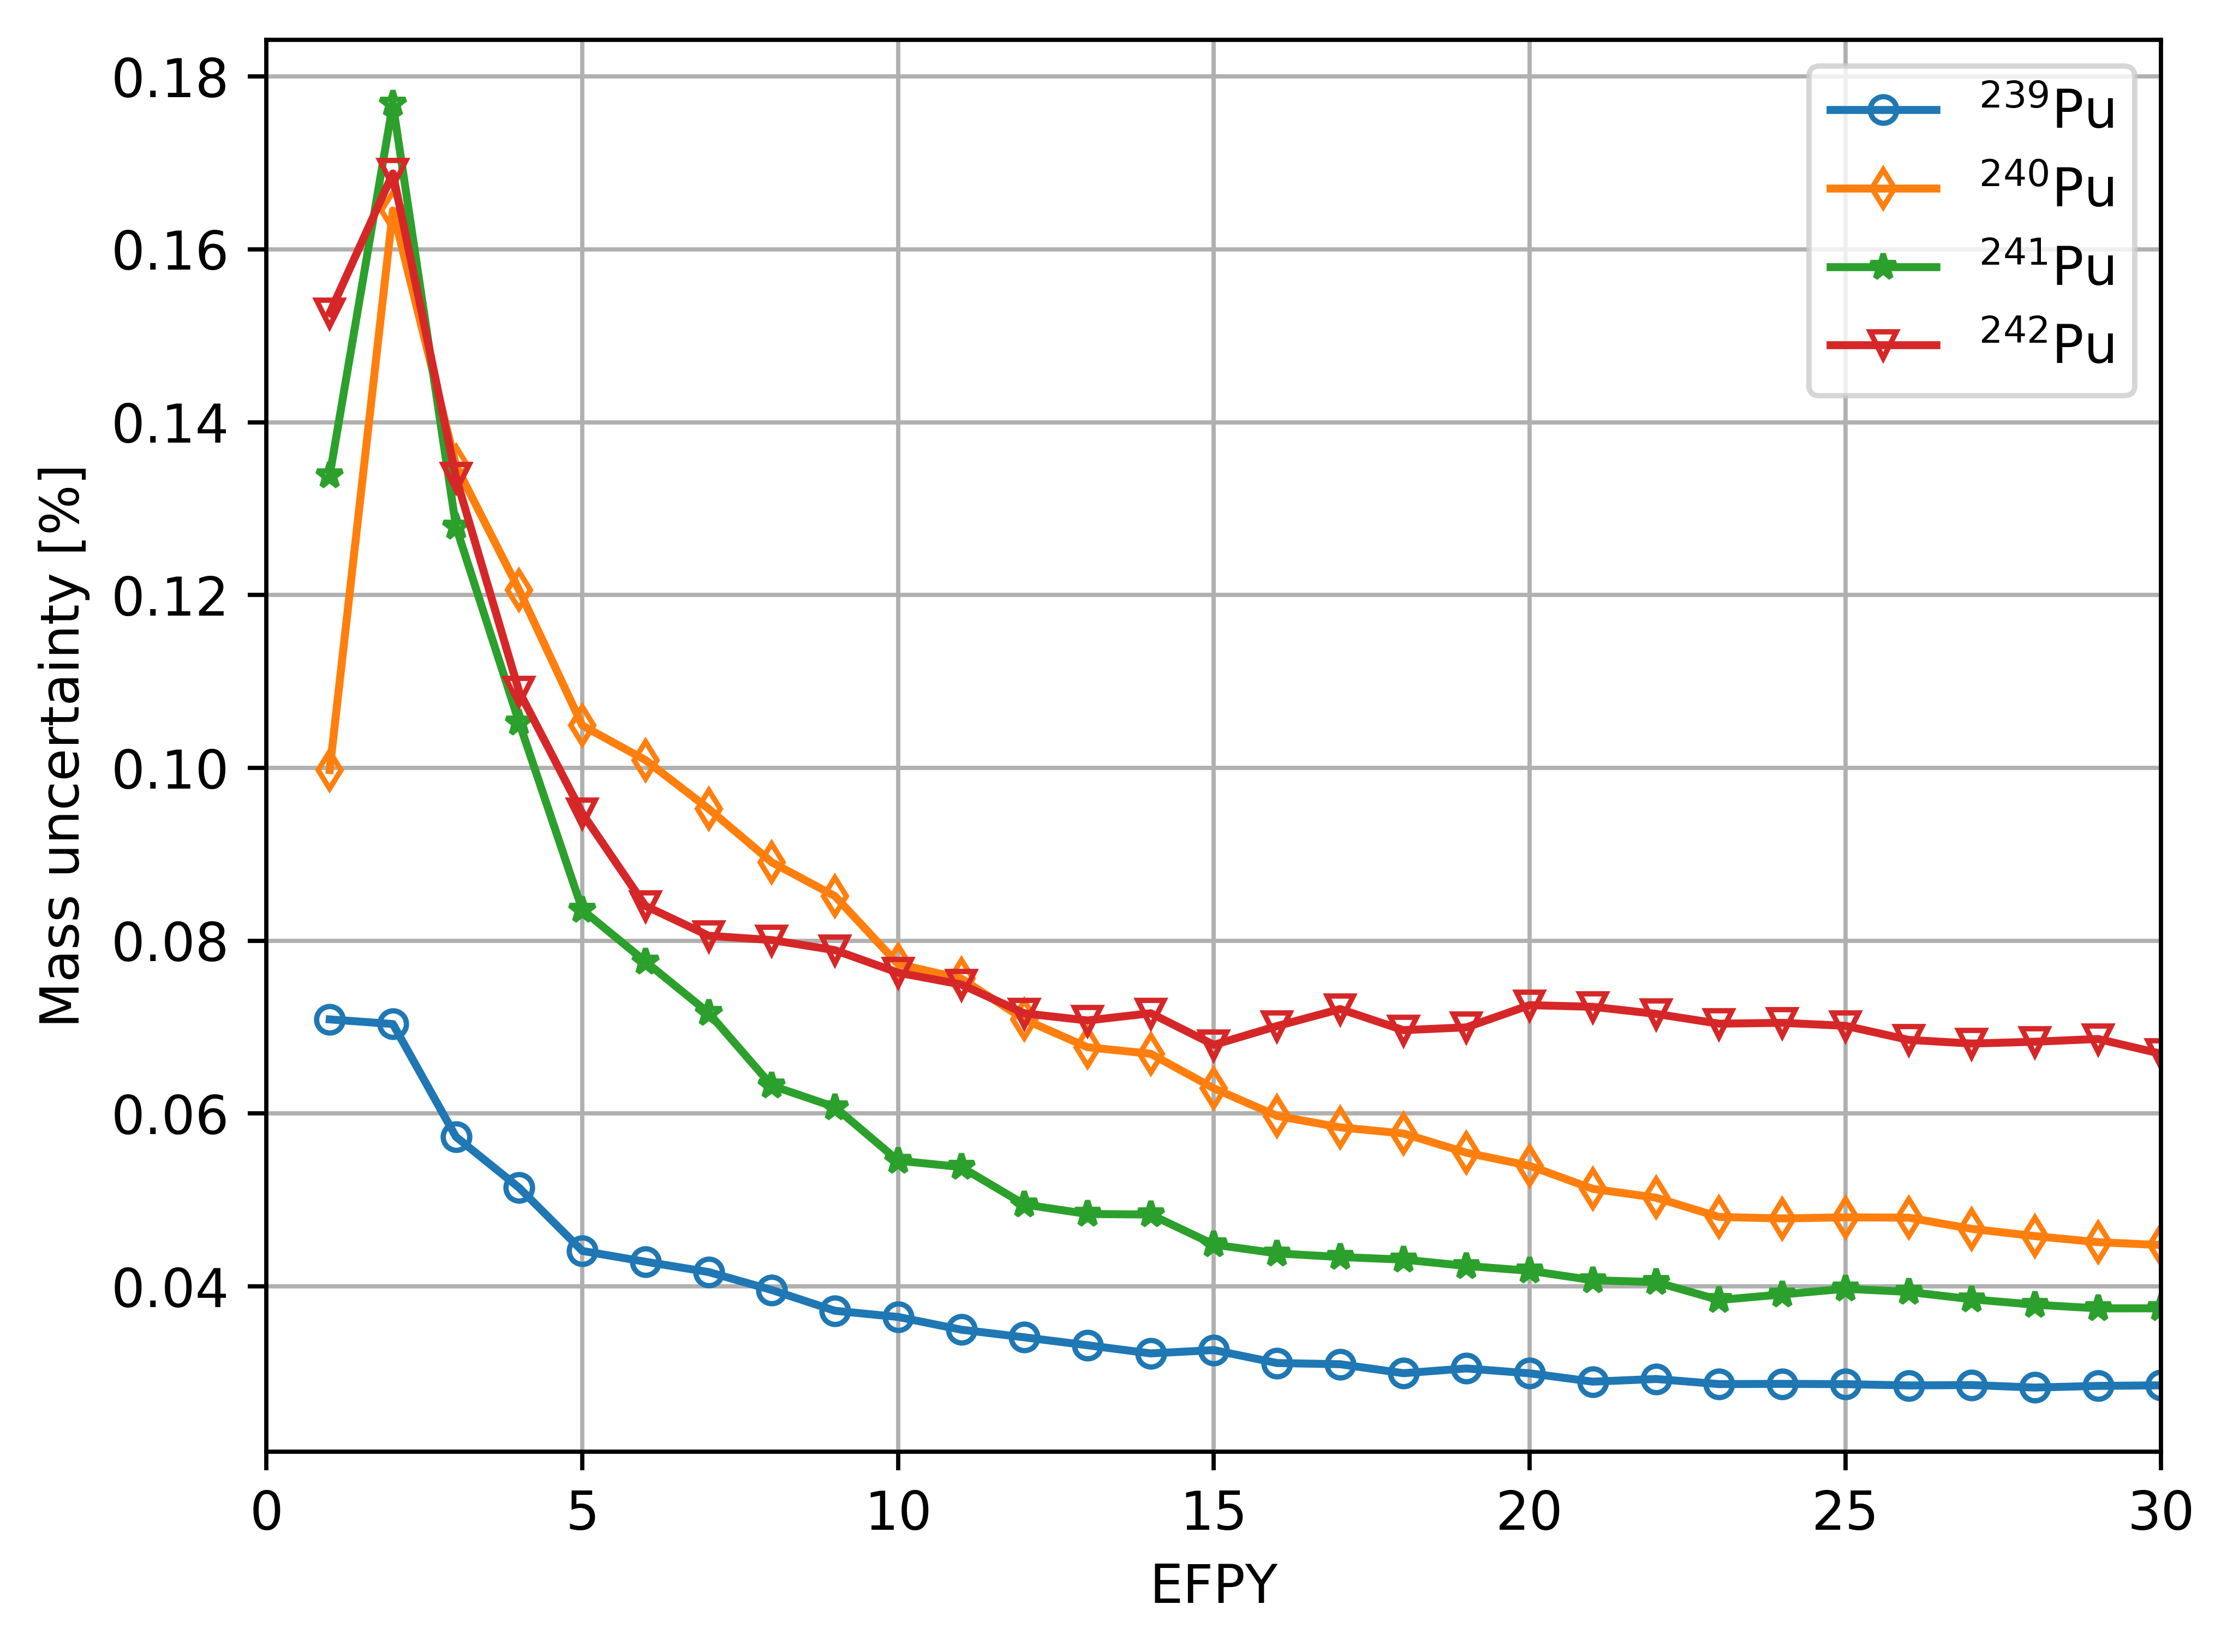
\includegraphics[width=0.8\textwidth]{uq/serpent_mass_std_pu.png}
	\caption{Caption here.}
	\label{fig:pu}
\end{figure}
\begin{figure}[hbp!] % replace 't' with 'b' to 
	\centering
	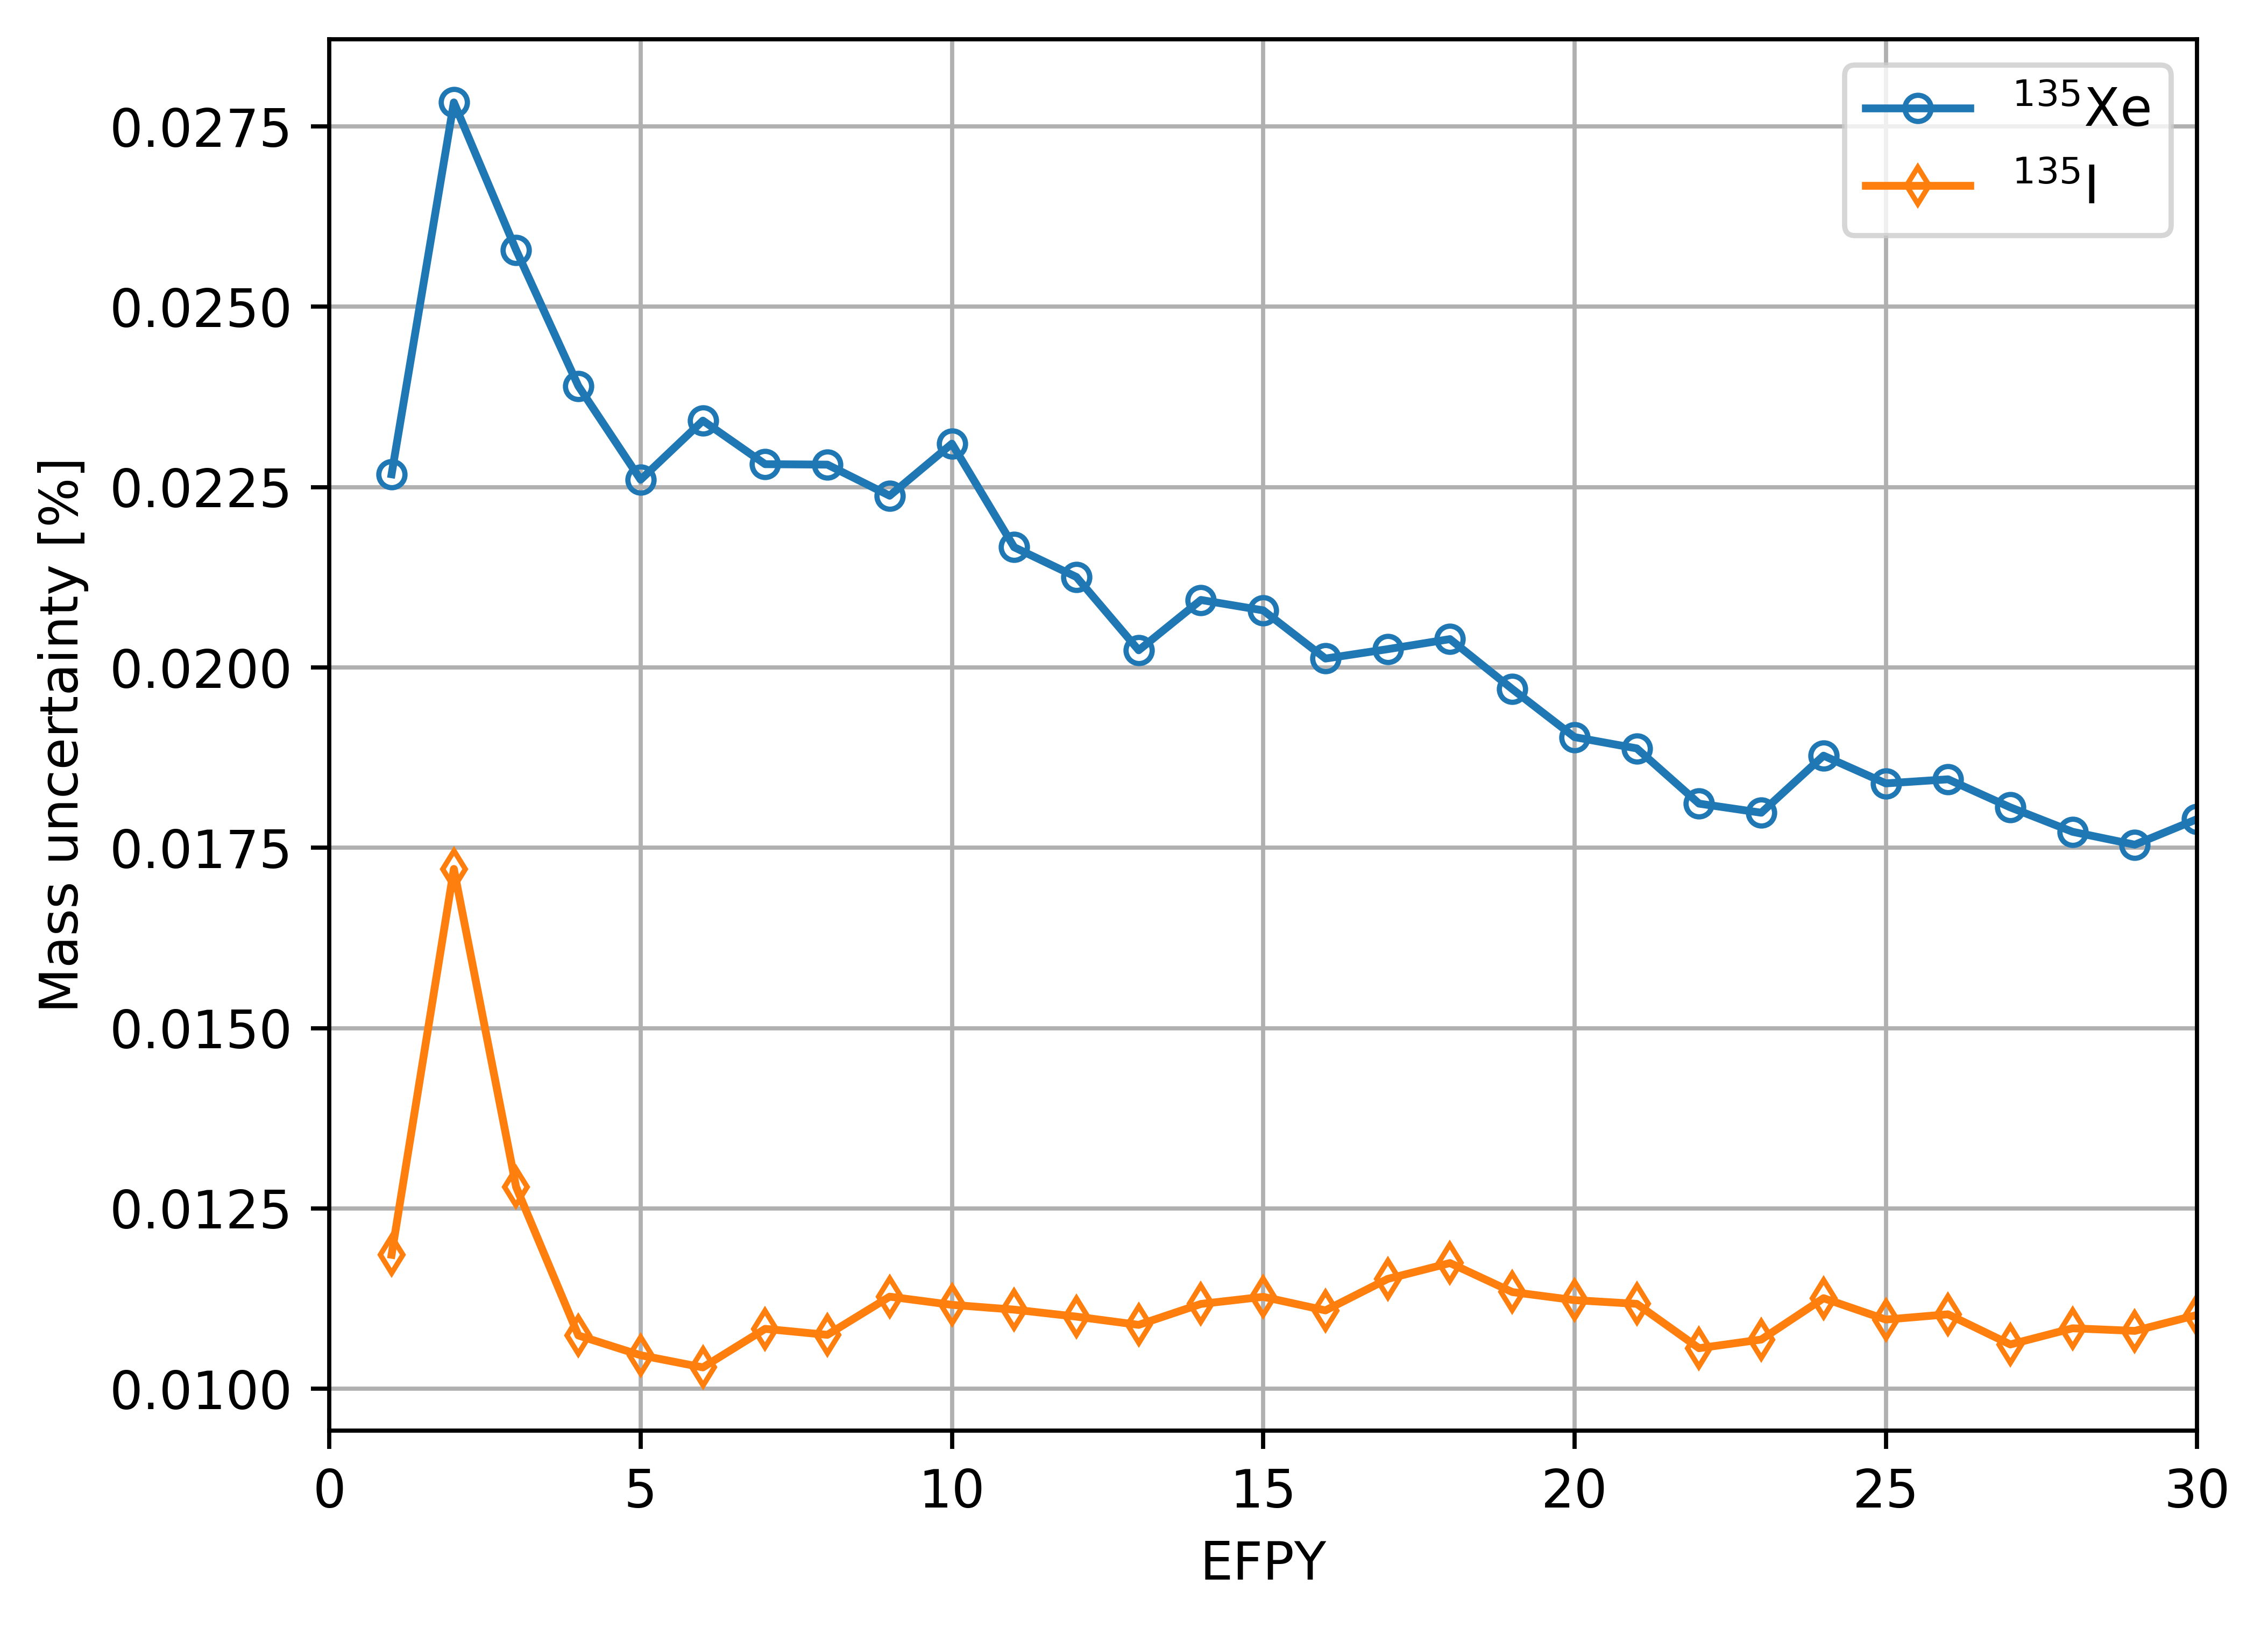
\includegraphics[width=0.8\textwidth]{uq/serpent_mass_std_xe_i.png}
	\caption{Caption here.}
	\label{fig:xe-i}
\end{figure}
\begin{figure}[hbp!] % replace 't' with 'b' to 
	\centering
	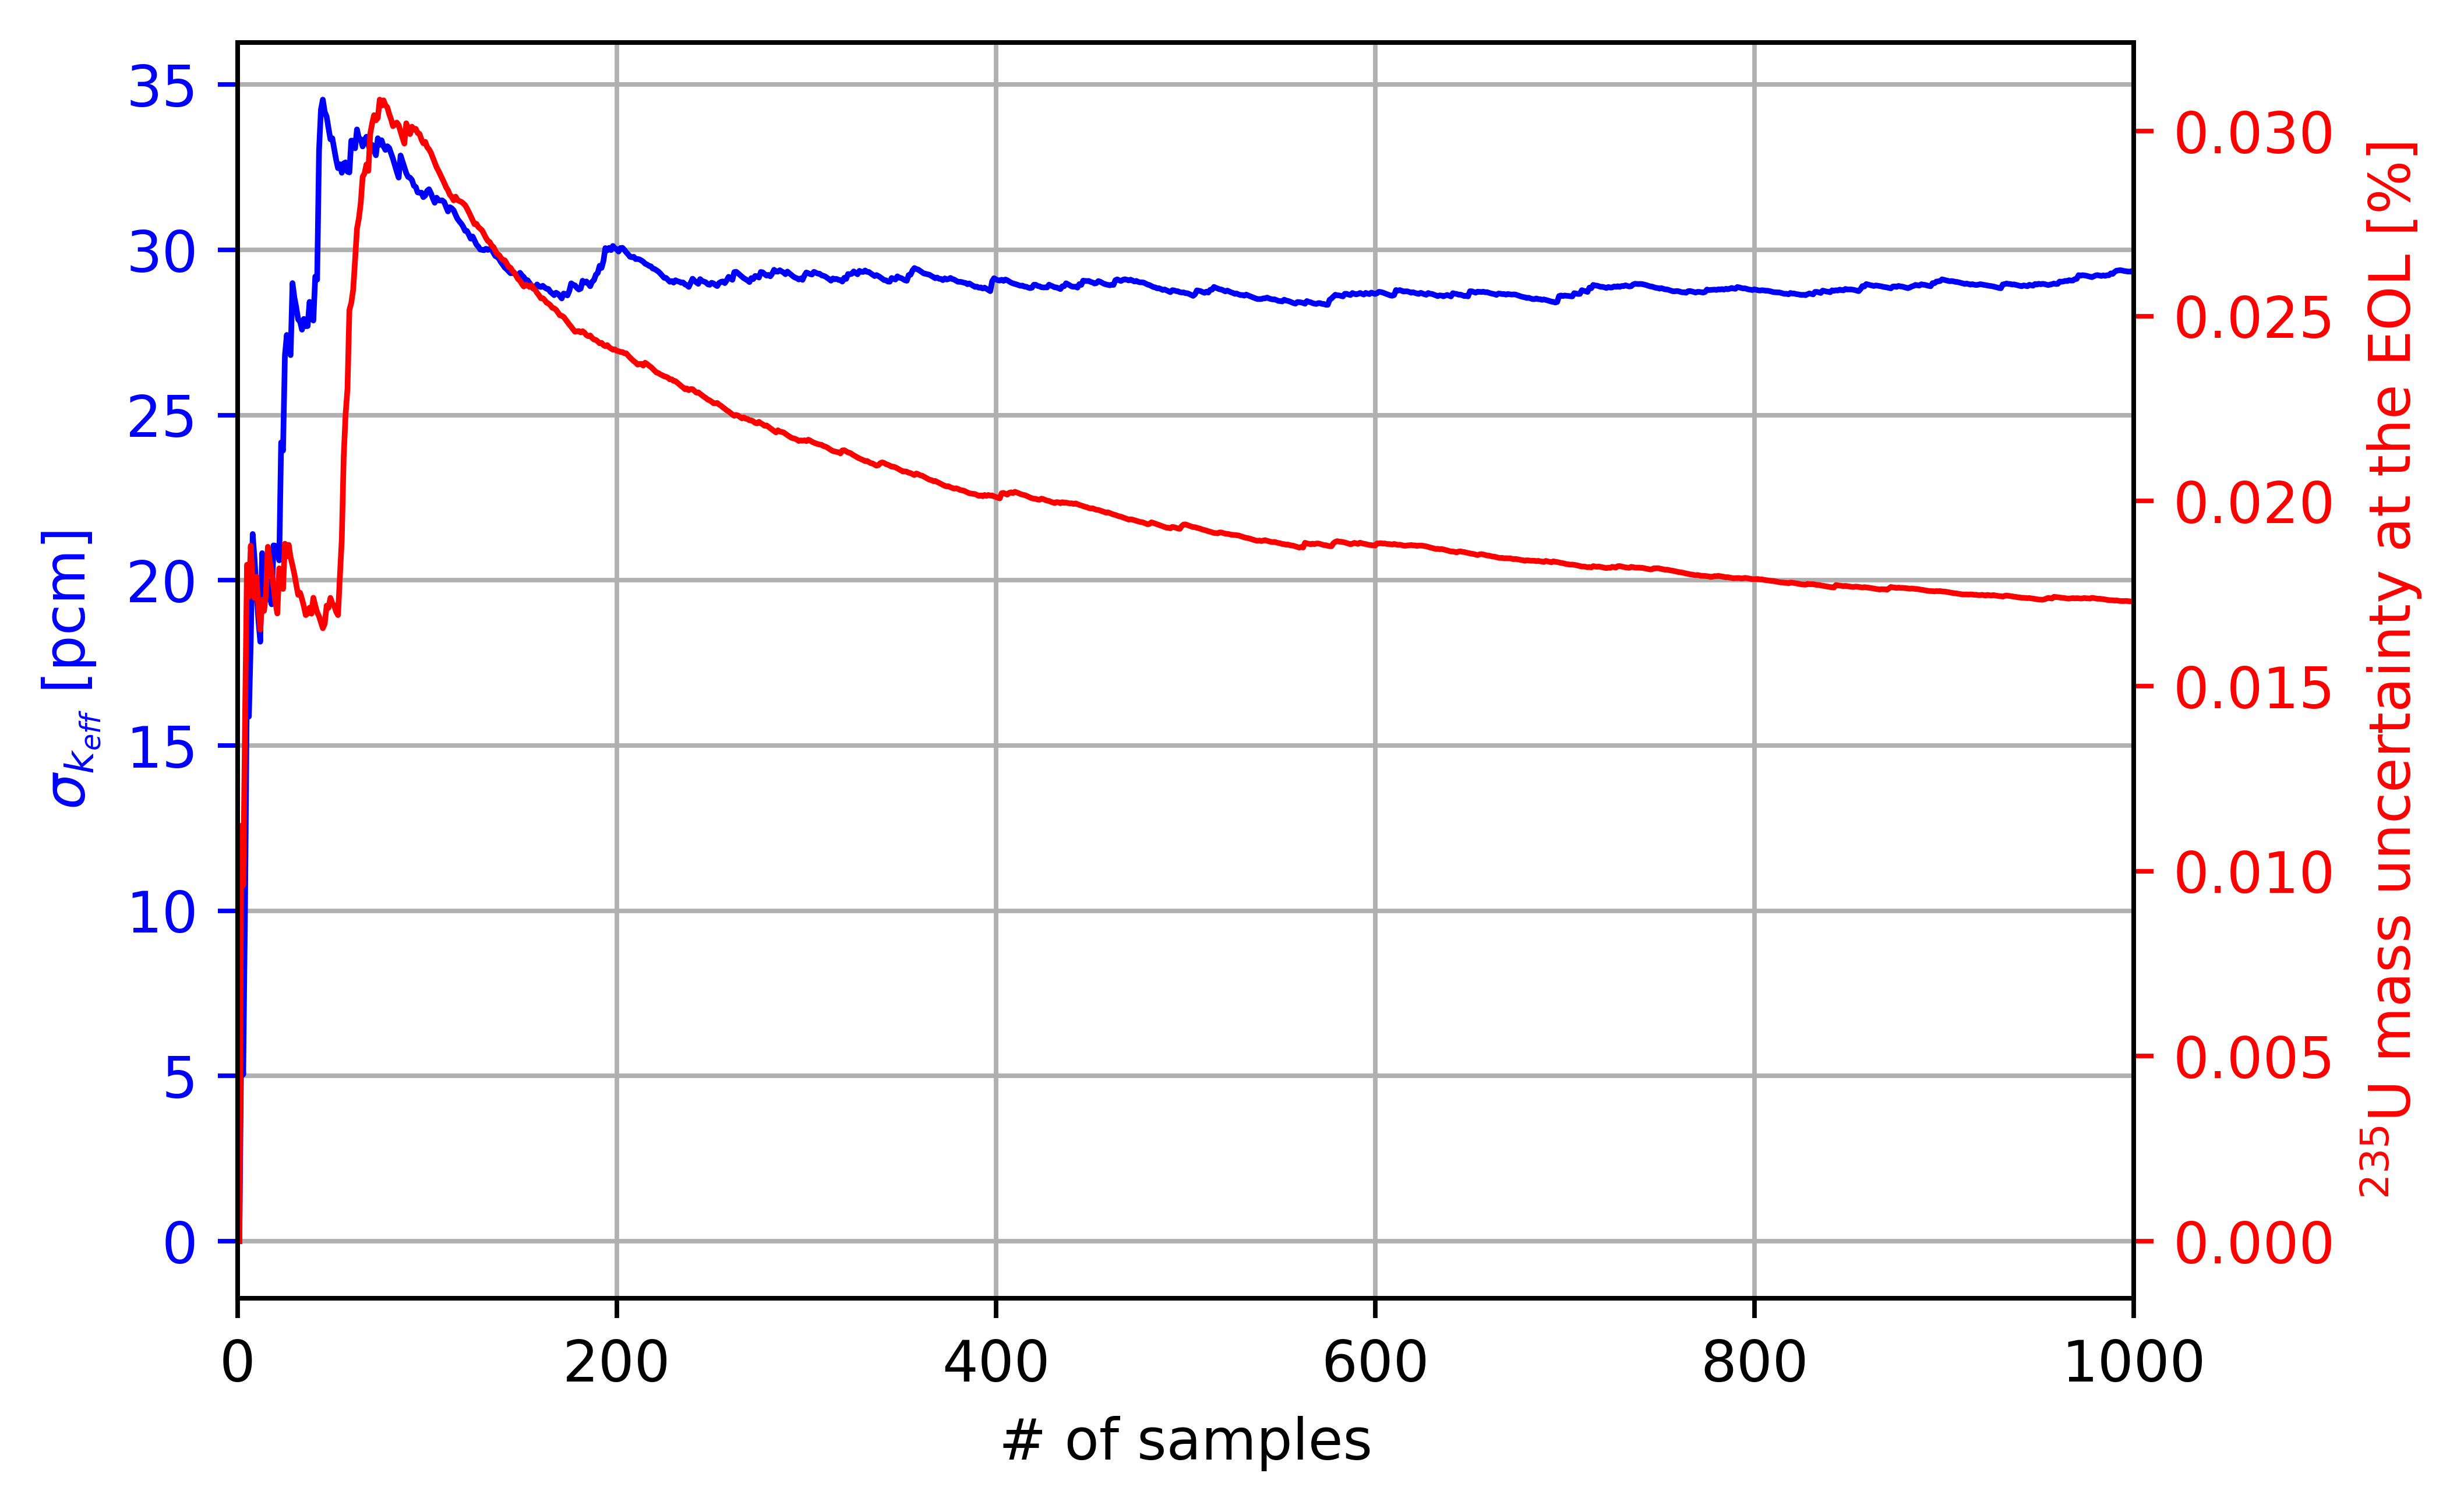
\includegraphics[width=0.8\textwidth]{uq/serpent_convergance_for_tap.png}
	\caption{Caption here.}
	\label{fig:uq-convergance}
\end{figure}

\section{Nuclear data related uncertainty in depleted fuel composition}
\begin{figure}[hbp!] % replace 't' with 'b' to 
	\centering
	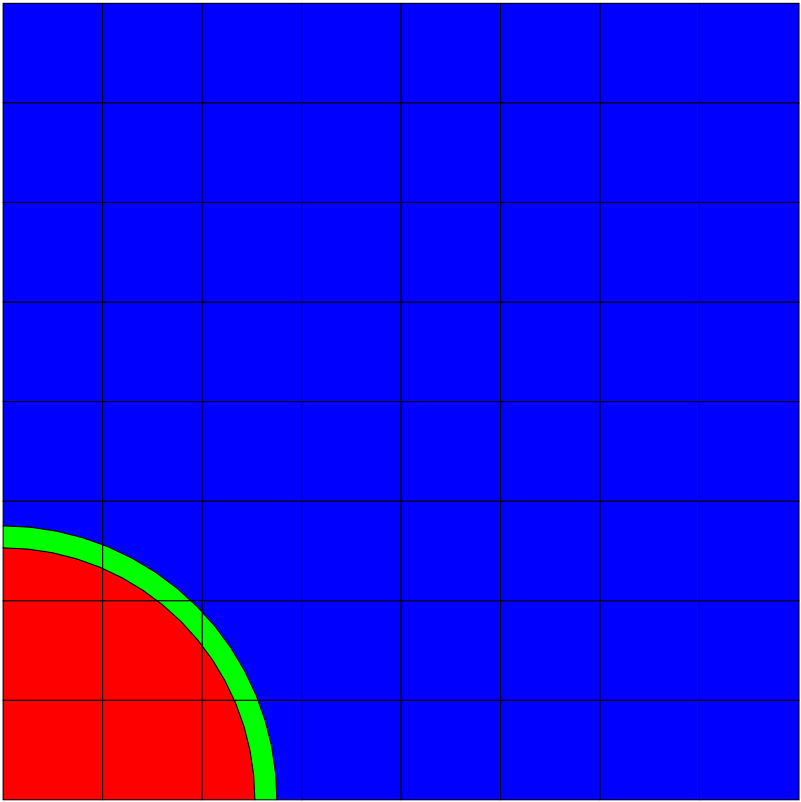
\includegraphics[width=0.8\textwidth]{uq/tap_pin_for_scale.png}
	\caption{Caption here.}
	\label{fig:uq-tap-pincell}
\end{figure}
\begin{figure}[hbp!] % replace 't' with 'b' to 
	\centering
	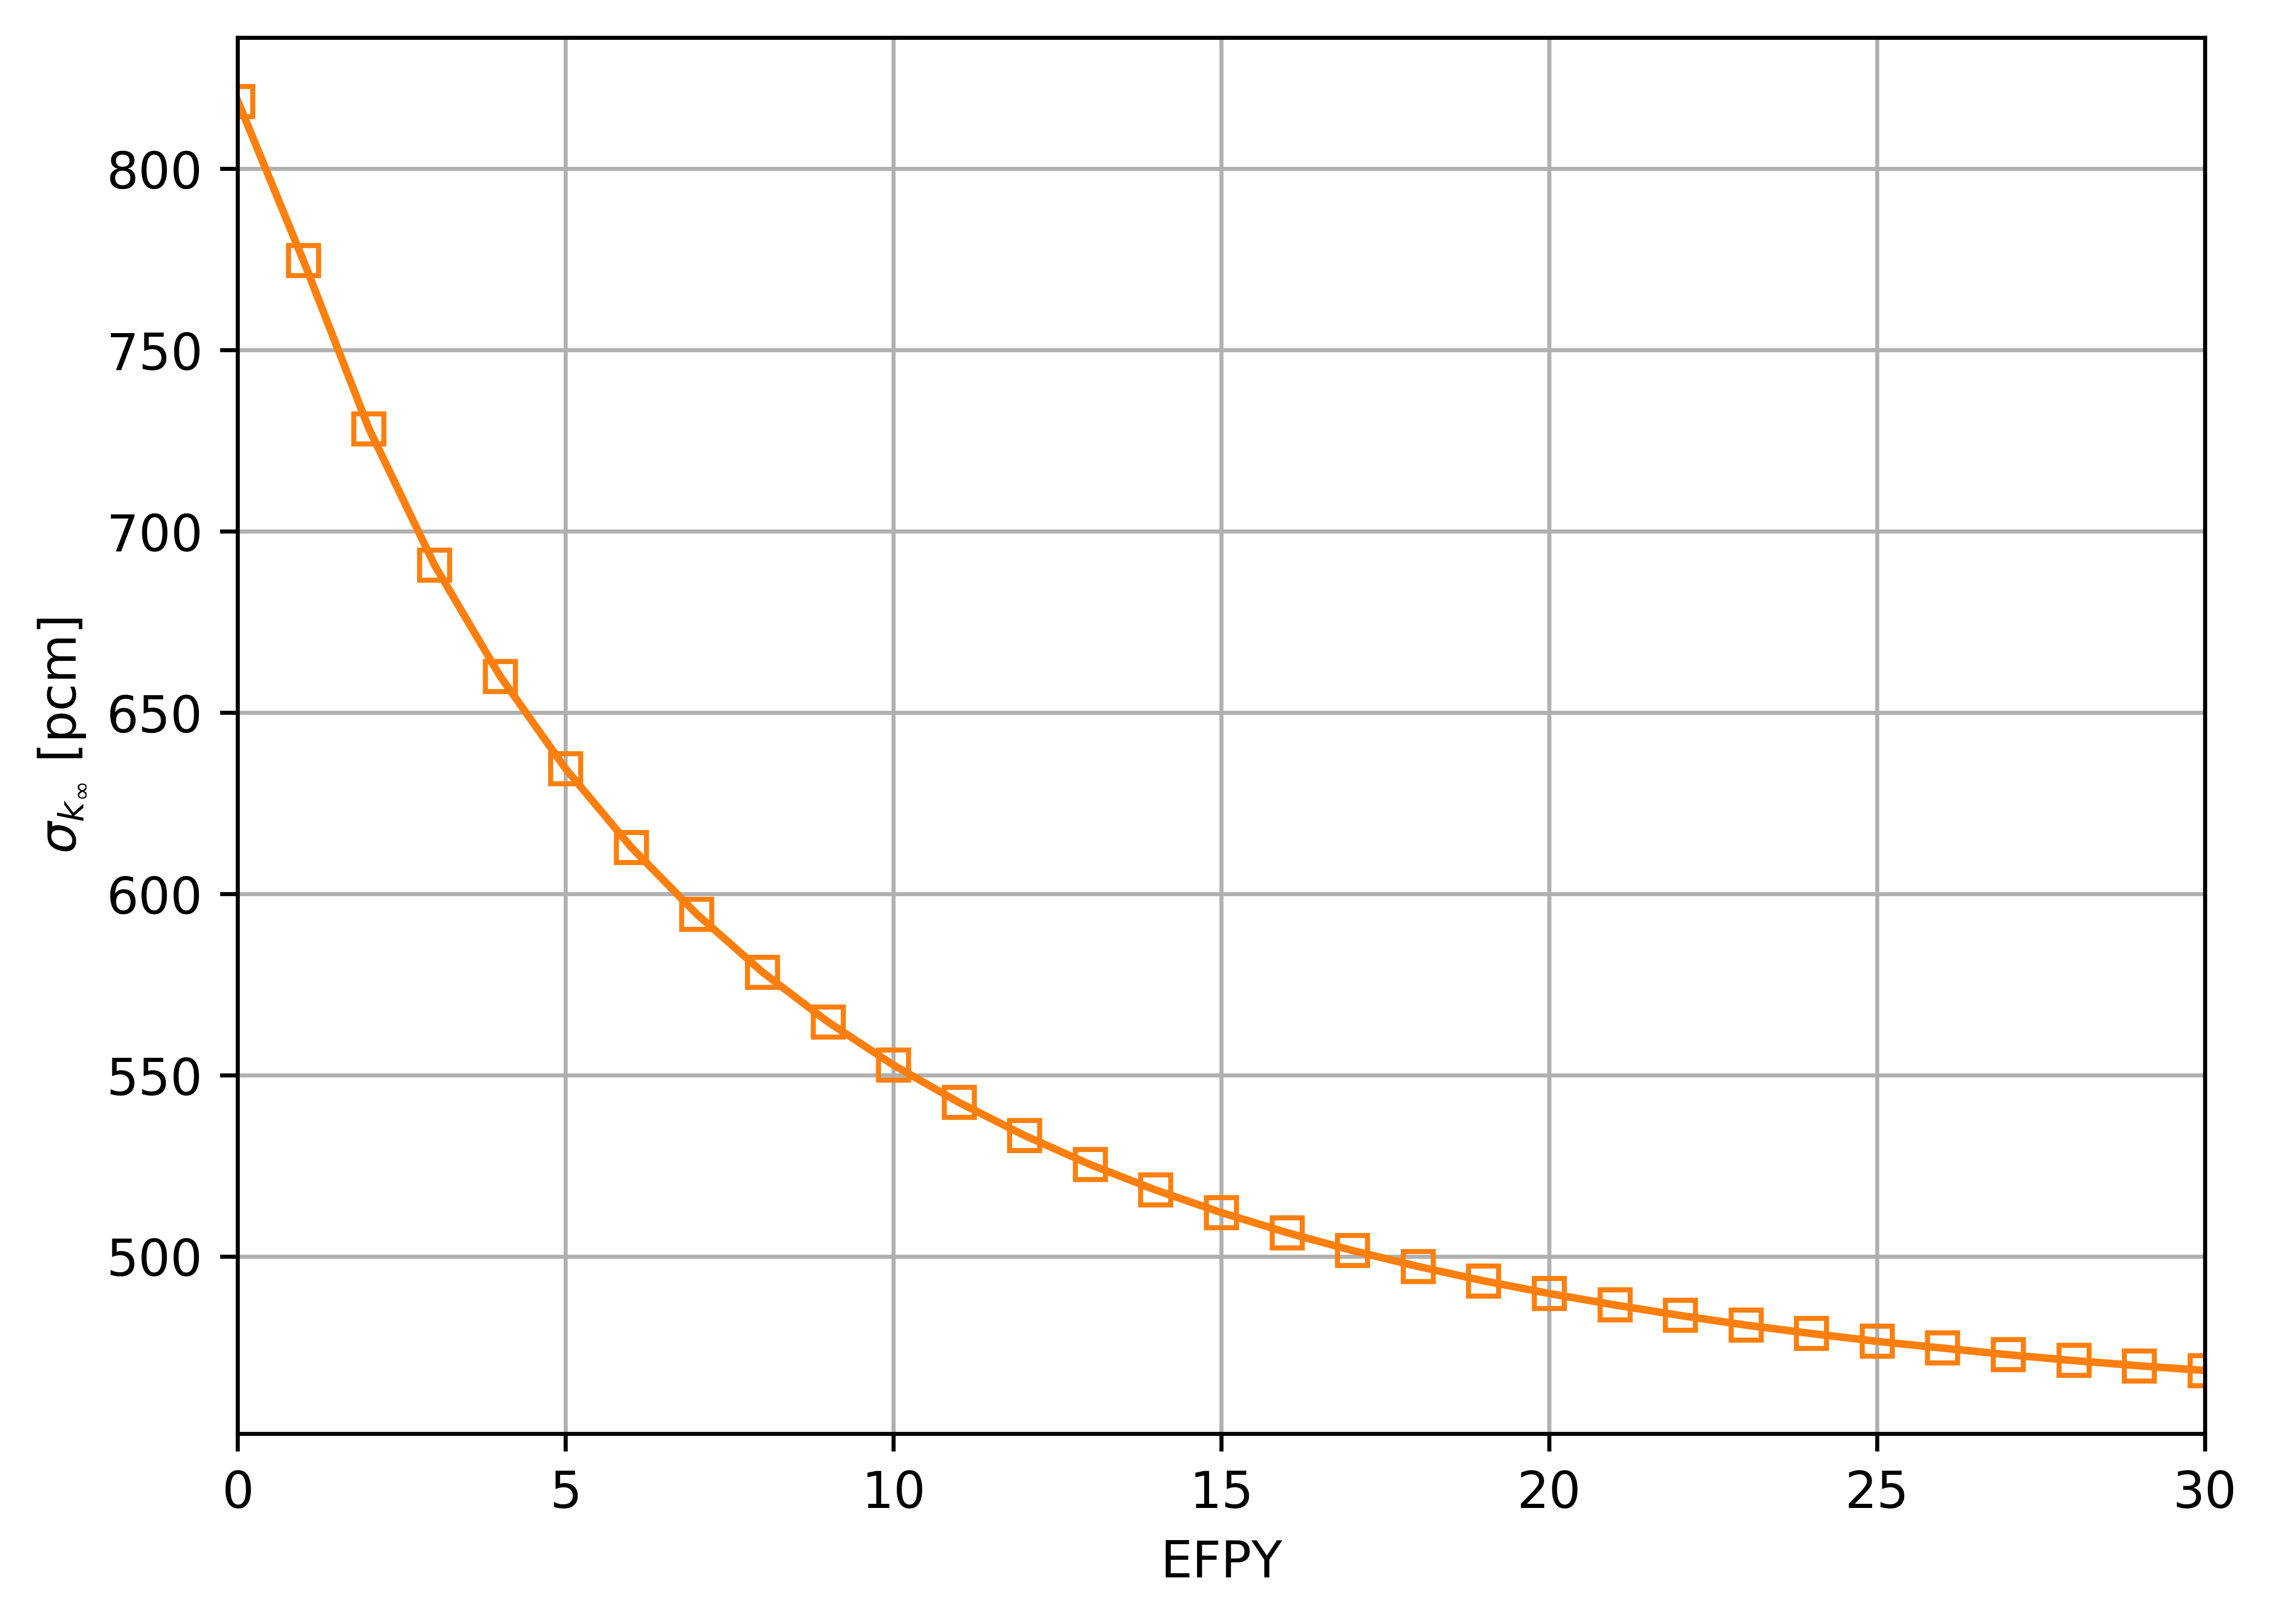
\includegraphics[width=0.8\textwidth]{uq/scale_kinf_dynamics_for_tap.png}
	\caption{Caption here.}
	\label{fig:uq-scale-kinf}
\end{figure}
\begin{figure}[hbp!] % replace 't' with 'b' to 
	\centering
	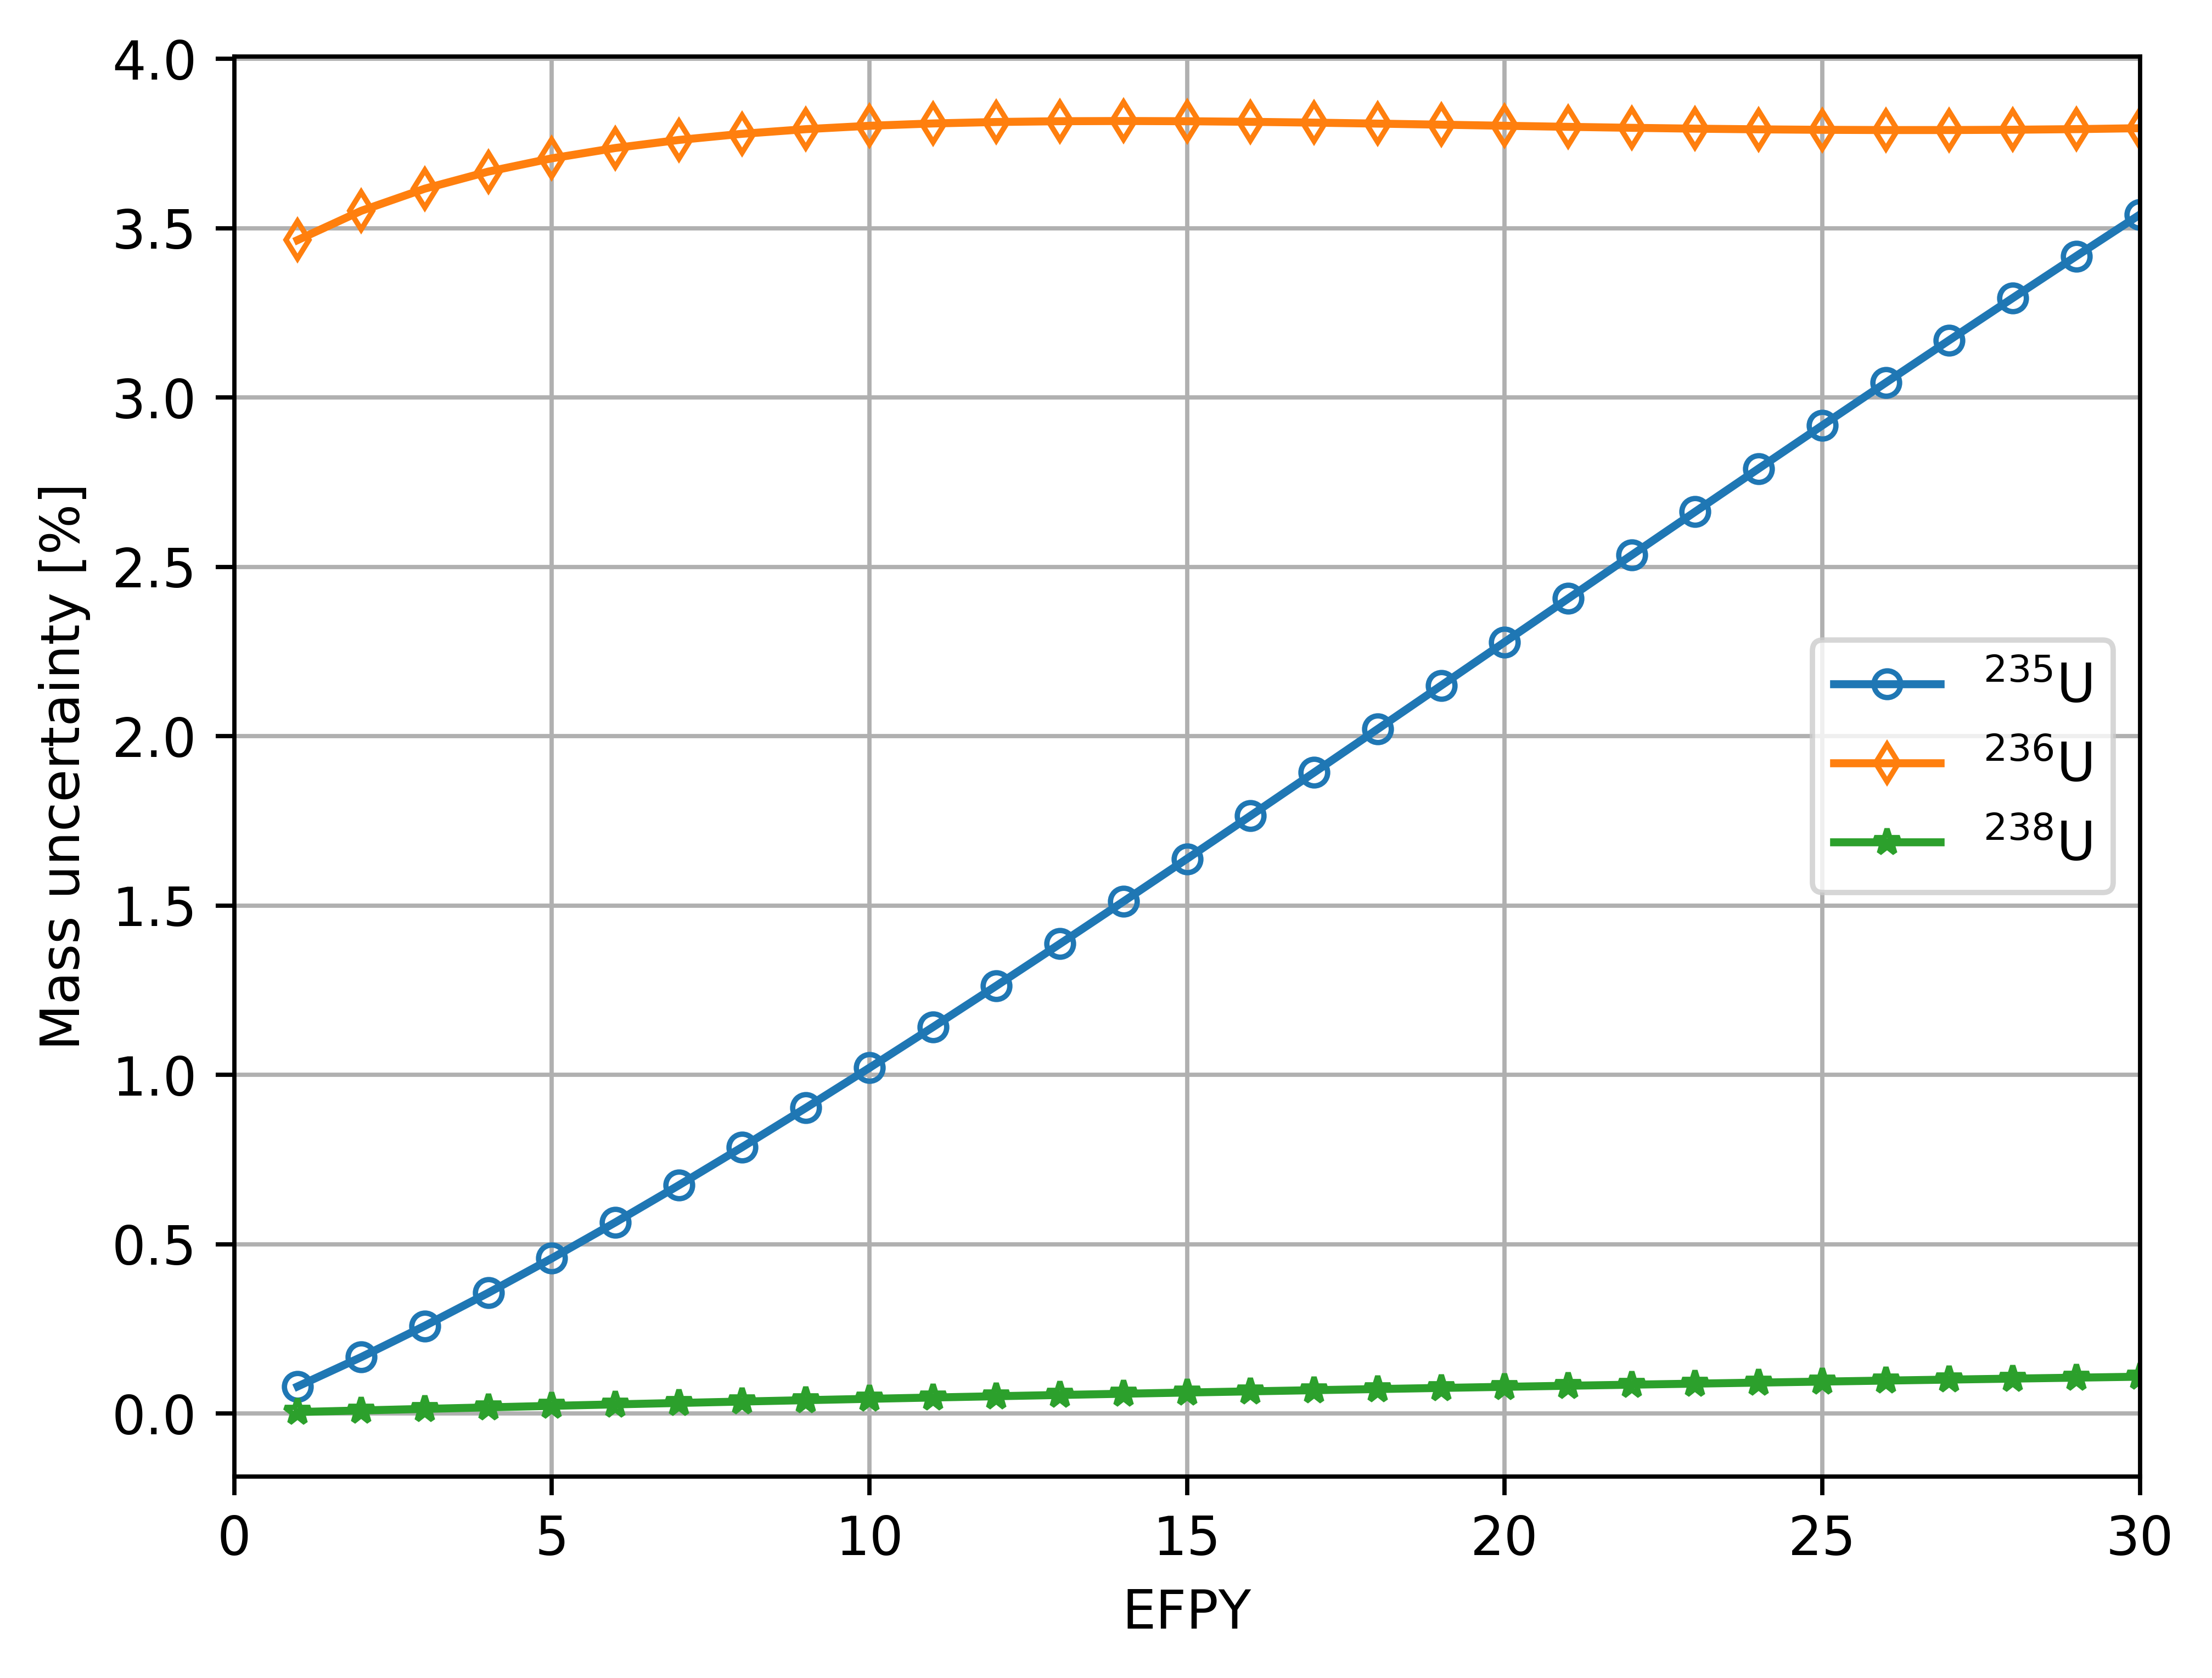
\includegraphics[width=0.8\textwidth]{uq/scale_mass_std_u.png}
	\caption{Caption here.}
	\label{fig:uq-scale-u}
\end{figure}

\begin{figure}[hbp!] % replace 't' with 'b' to 
	\centering
	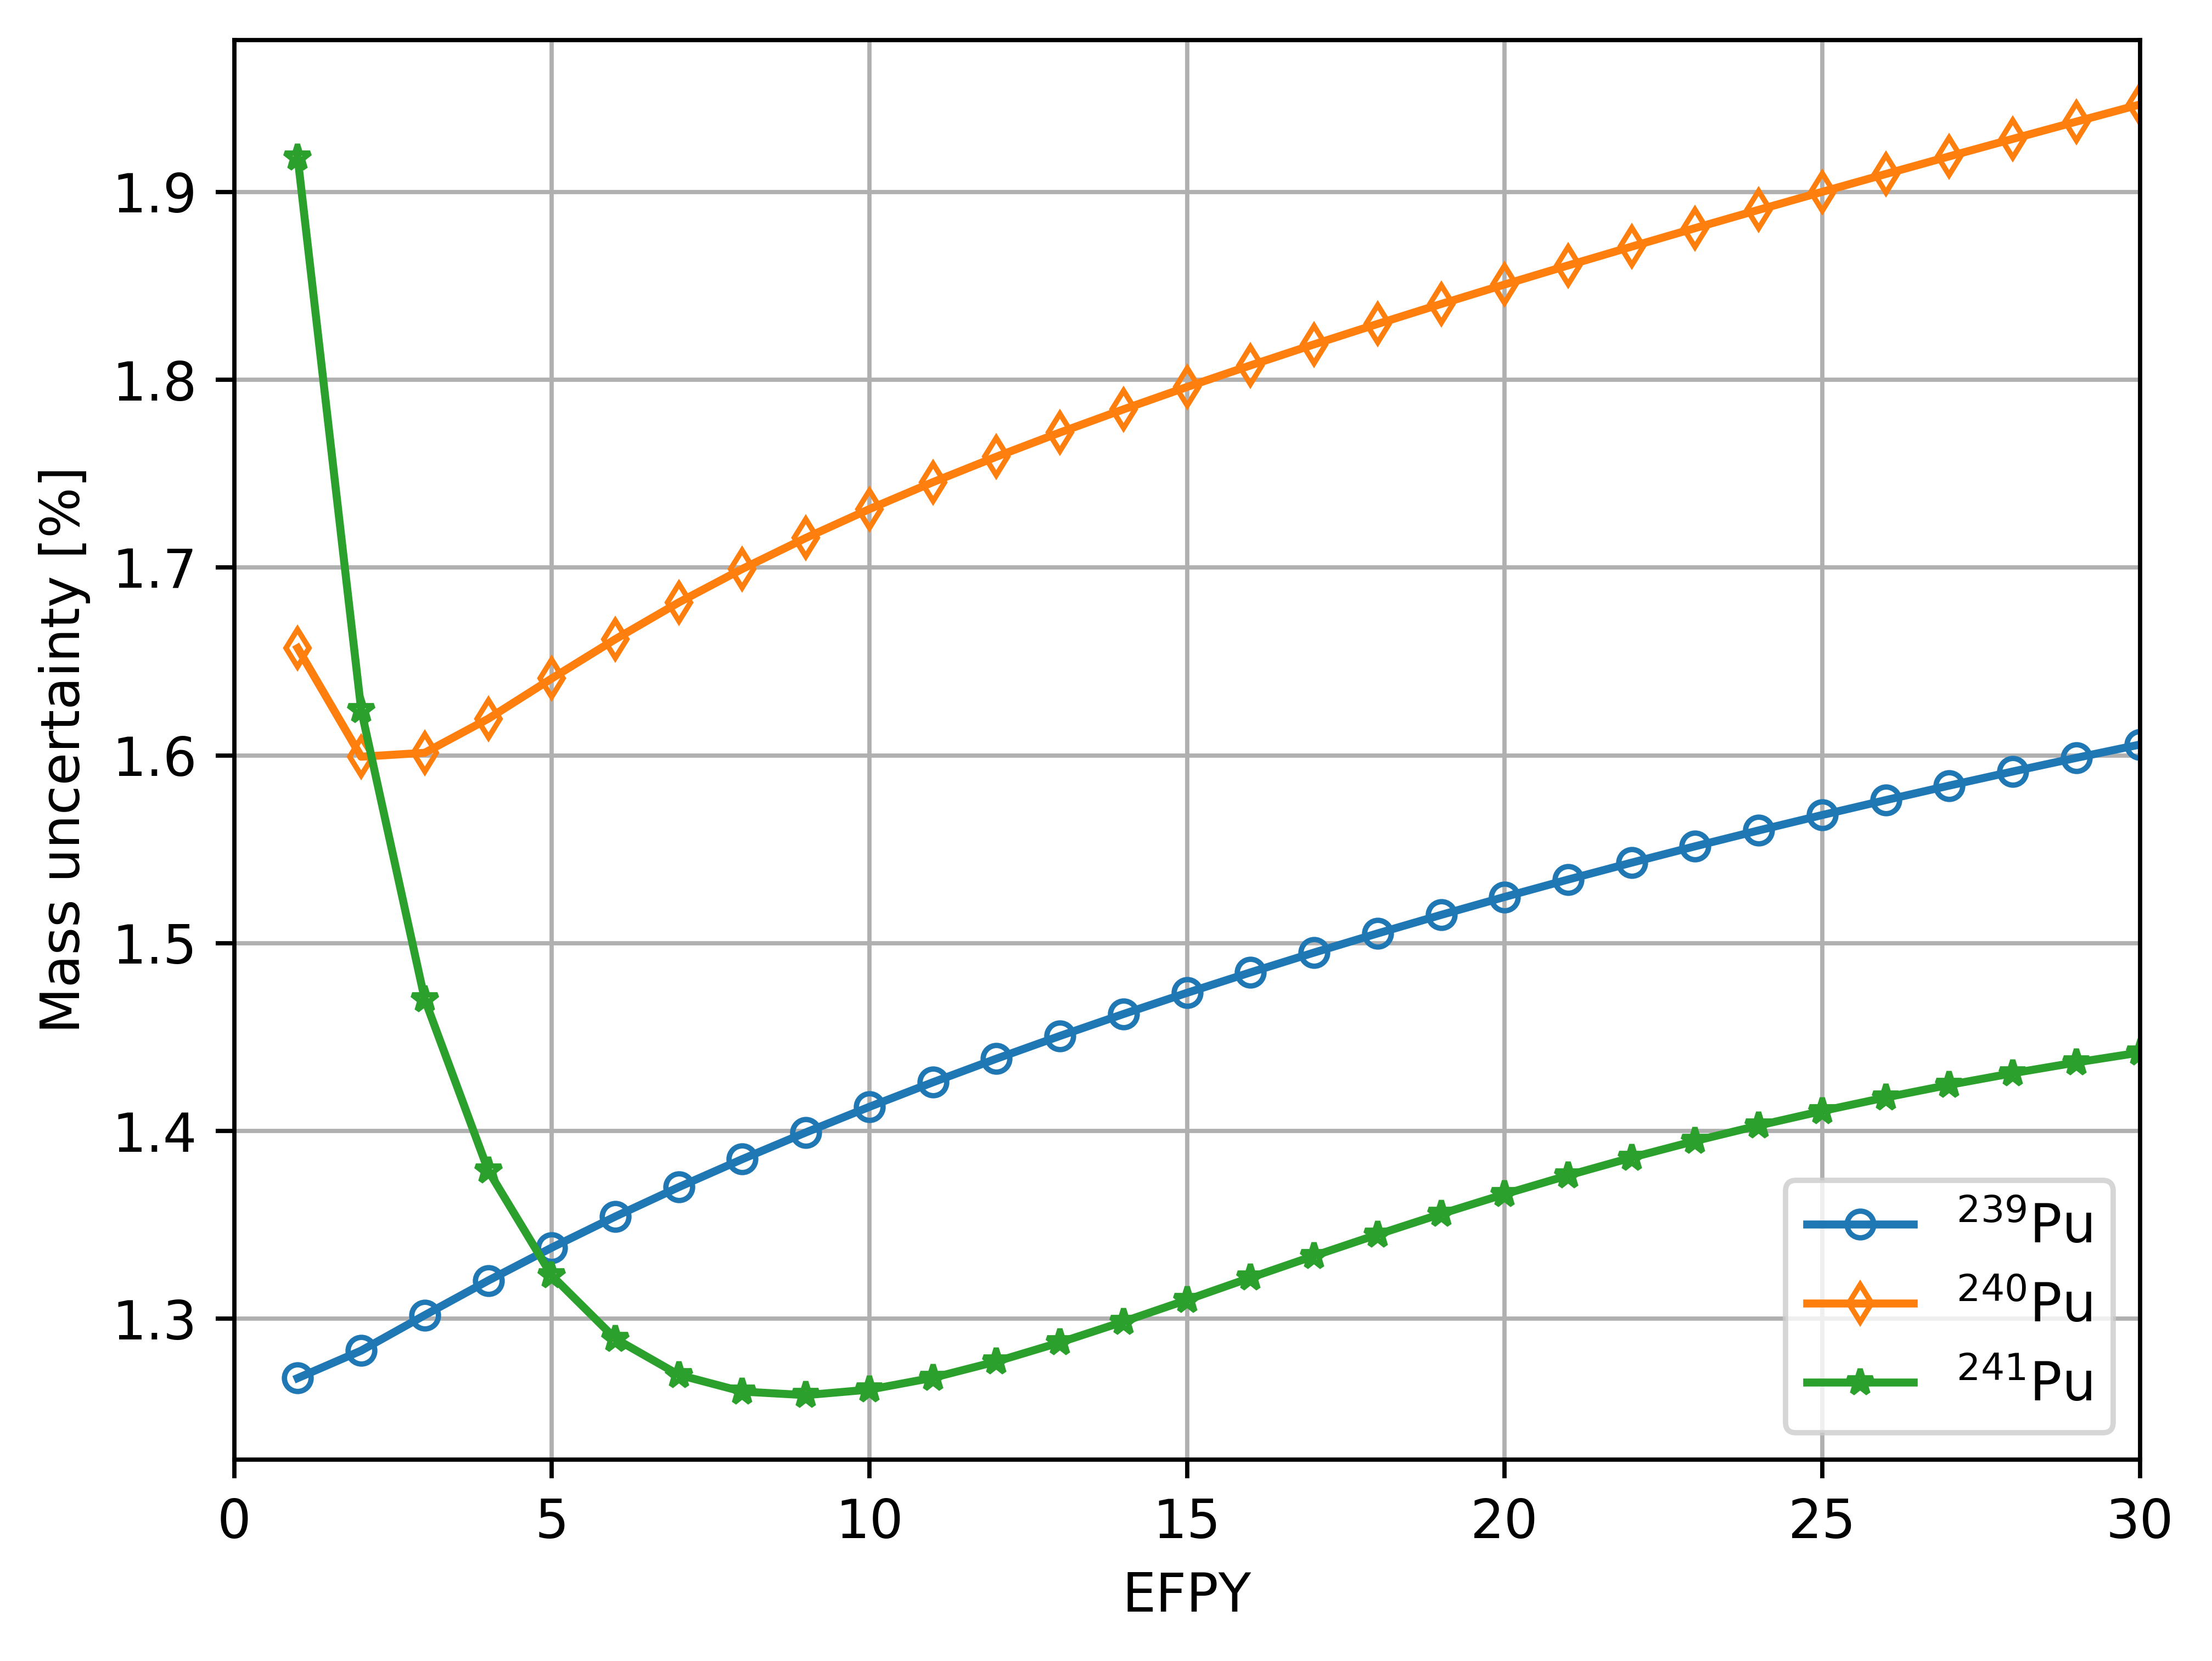
\includegraphics[width=0.8\textwidth]{uq/scale_mass_std_pu.png}
	\caption{Caption here.}
	\label{fig:uq-scale-pu}
\end{figure}

\begin{figure}[hbp!] % replace 't' with 'b' to 
	\centering
	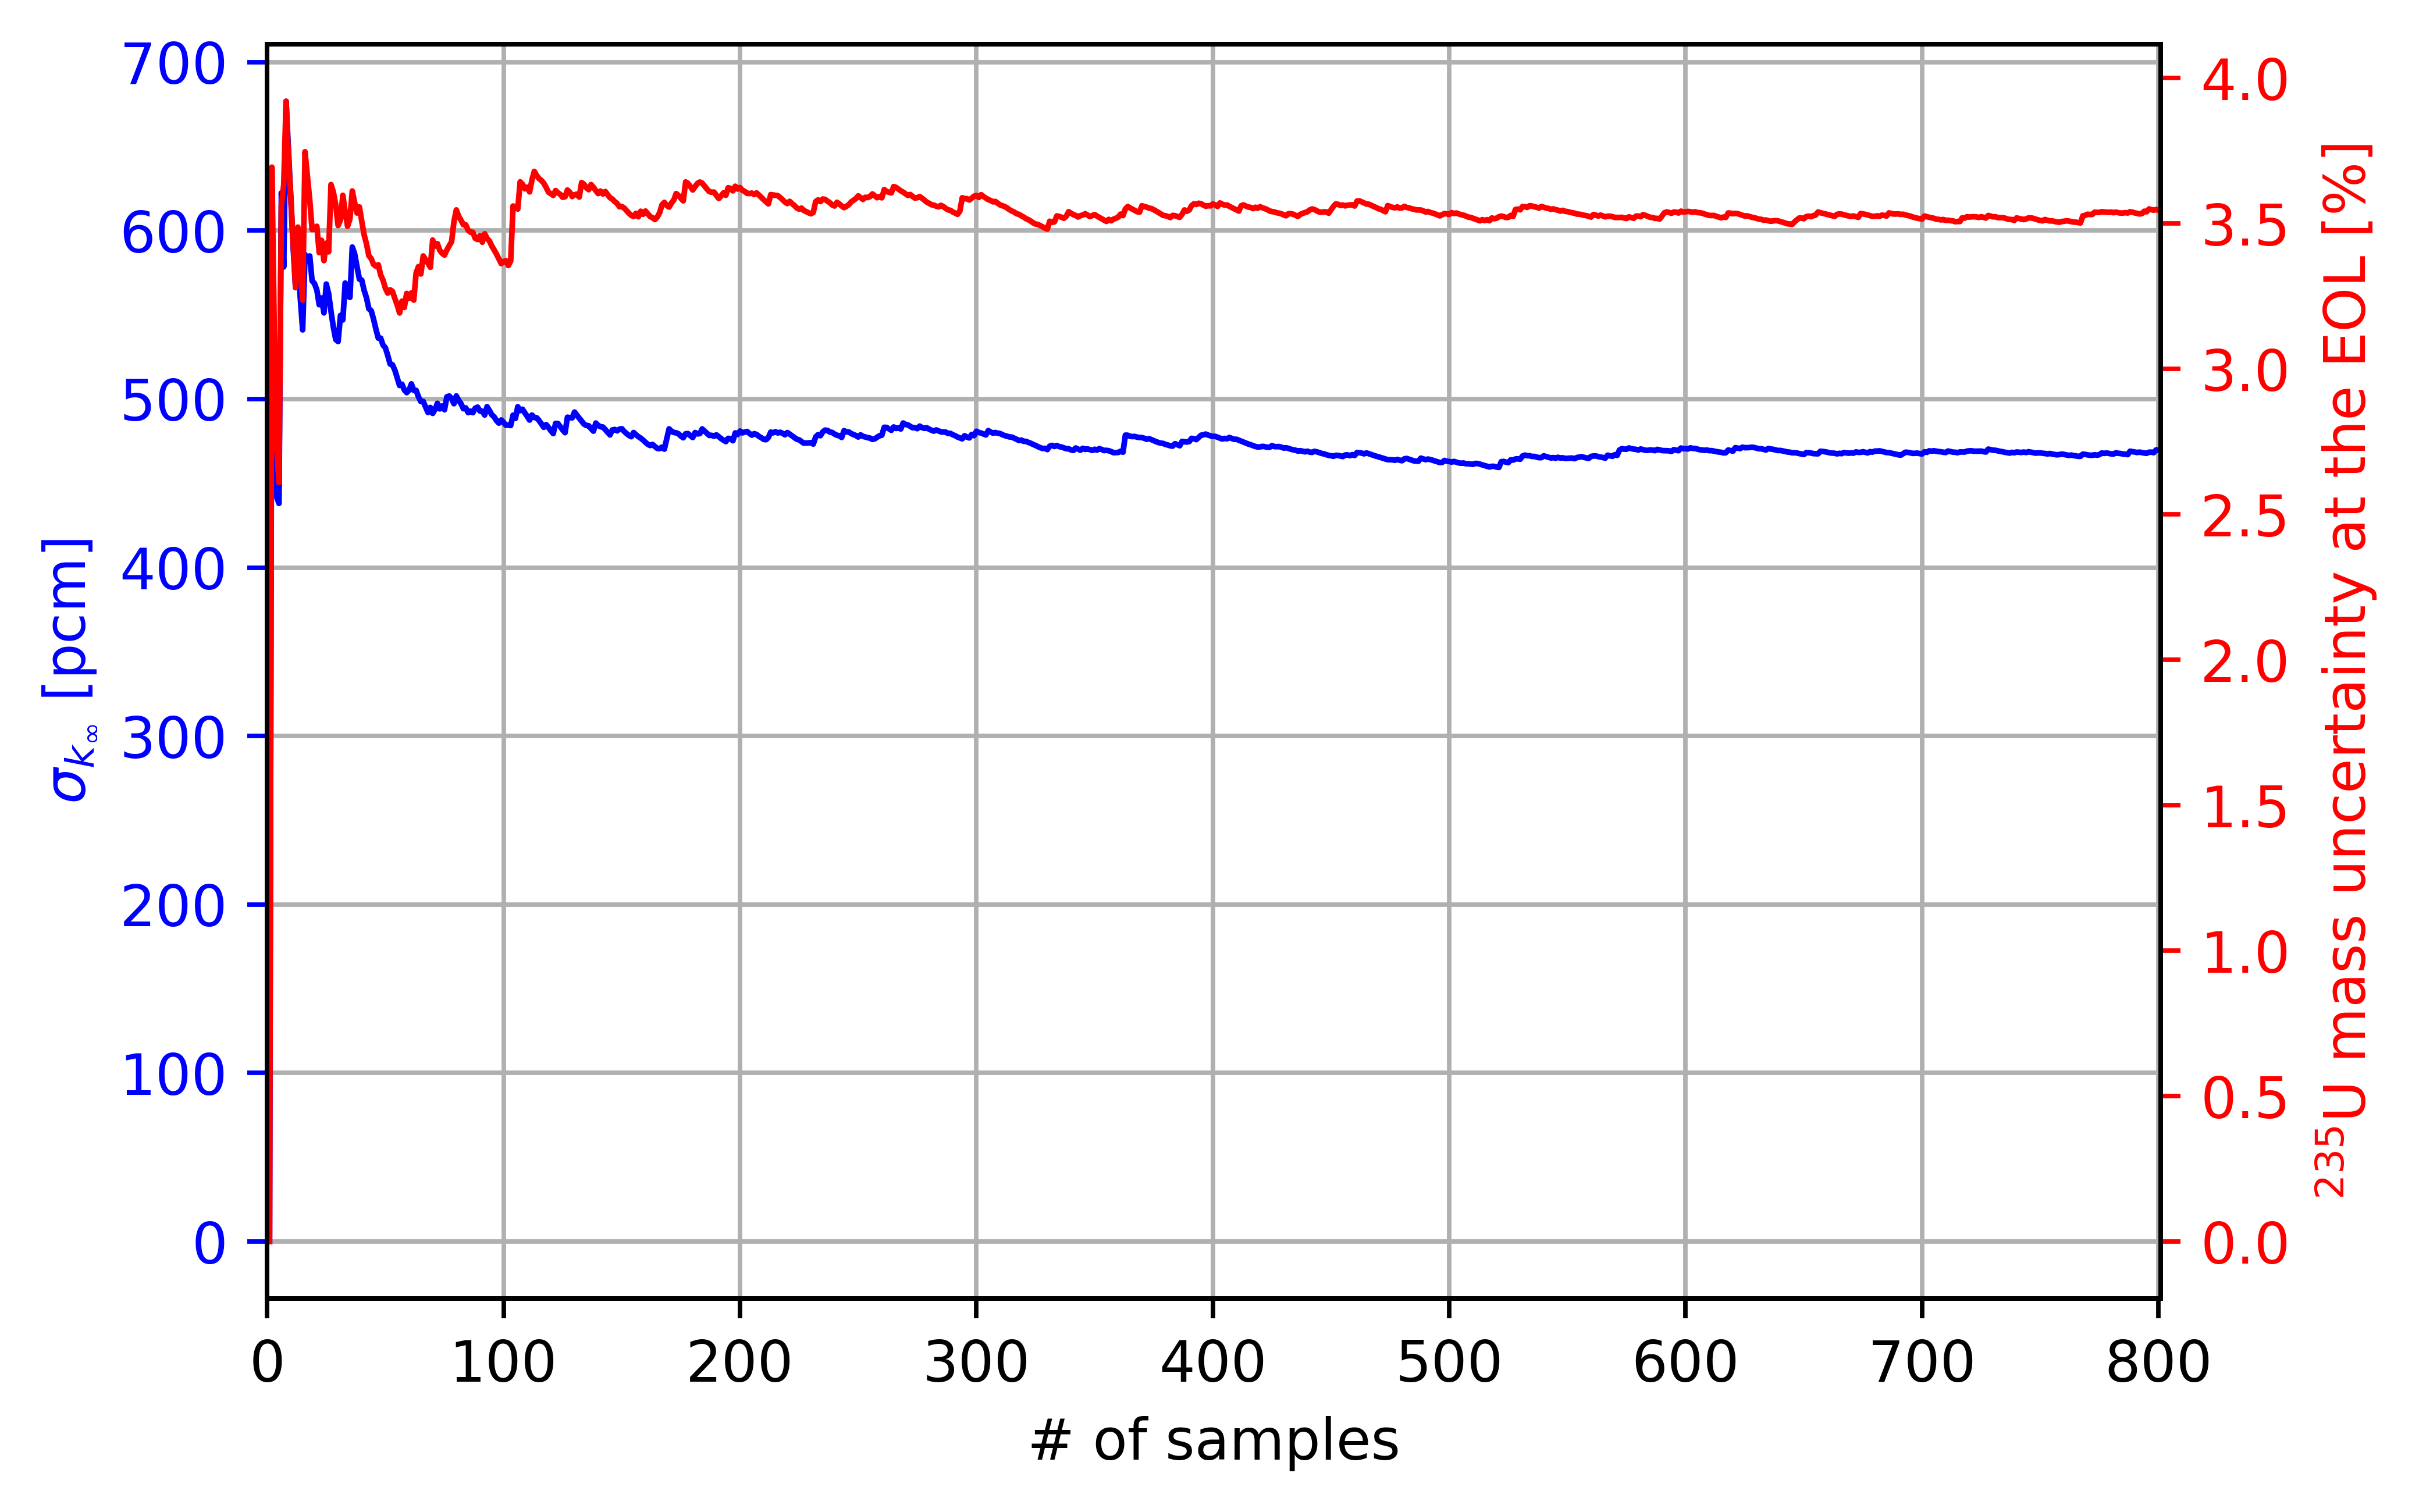
\includegraphics[width=0.8\textwidth]{uq/scale_convergance_for_tap.png}
	\caption{Caption here.}
	\label{fig:uq-scale-convergance}
\end{figure}

\section{Concluding remarks}